\PassOptionsToPackage{unicode=true}{hyperref} % options for packages loaded elsewhere
\PassOptionsToPackage{hyphens}{url}
%
\documentclass[]{article}
\usepackage{lmodern}
\usepackage{amssymb,amsmath}
\usepackage{ifxetex,ifluatex}
\usepackage{fixltx2e} % provides \textsubscript
\ifnum 0\ifxetex 1\fi\ifluatex 1\fi=0 % if pdftex
  \usepackage[T1]{fontenc}
  \usepackage[utf8]{inputenc}
  \usepackage{textcomp} % provides euro and other symbols
\else % if luatex or xelatex
  \usepackage{unicode-math}
  \defaultfontfeatures{Ligatures=TeX,Scale=MatchLowercase}
\fi
% use upquote if available, for straight quotes in verbatim environments
\IfFileExists{upquote.sty}{\usepackage{upquote}}{}
% use microtype if available
\IfFileExists{microtype.sty}{%
\usepackage[]{microtype}
\UseMicrotypeSet[protrusion]{basicmath} % disable protrusion for tt fonts
}{}
\IfFileExists{parskip.sty}{%
\usepackage{parskip}
}{% else
\setlength{\parindent}{0pt}
\setlength{\parskip}{6pt plus 2pt minus 1pt}
}
\usepackage{hyperref}
\hypersetup{
            pdftitle={SOMDisco},
            pdfauthor={Josh Taylor},
            pdfborder={0 0 0},
            breaklinks=true}
\urlstyle{same}  % don't use monospace font for urls
\usepackage{color}
\usepackage{fancyvrb}
\newcommand{\VerbBar}{|}
\newcommand{\VERB}{\Verb[commandchars=\\\{\}]}
\DefineVerbatimEnvironment{Highlighting}{Verbatim}{commandchars=\\\{\}}
% Add ',fontsize=\small' for more characters per line
\usepackage{framed}
\definecolor{shadecolor}{RGB}{248,248,248}
\newenvironment{Shaded}{\begin{snugshade}}{\end{snugshade}}
\newcommand{\AlertTok}[1]{\textcolor[rgb]{0.94,0.16,0.16}{#1}}
\newcommand{\AnnotationTok}[1]{\textcolor[rgb]{0.56,0.35,0.01}{\textbf{\textit{#1}}}}
\newcommand{\AttributeTok}[1]{\textcolor[rgb]{0.77,0.63,0.00}{#1}}
\newcommand{\BaseNTok}[1]{\textcolor[rgb]{0.00,0.00,0.81}{#1}}
\newcommand{\BuiltInTok}[1]{#1}
\newcommand{\CharTok}[1]{\textcolor[rgb]{0.31,0.60,0.02}{#1}}
\newcommand{\CommentTok}[1]{\textcolor[rgb]{0.56,0.35,0.01}{\textit{#1}}}
\newcommand{\CommentVarTok}[1]{\textcolor[rgb]{0.56,0.35,0.01}{\textbf{\textit{#1}}}}
\newcommand{\ConstantTok}[1]{\textcolor[rgb]{0.00,0.00,0.00}{#1}}
\newcommand{\ControlFlowTok}[1]{\textcolor[rgb]{0.13,0.29,0.53}{\textbf{#1}}}
\newcommand{\DataTypeTok}[1]{\textcolor[rgb]{0.13,0.29,0.53}{#1}}
\newcommand{\DecValTok}[1]{\textcolor[rgb]{0.00,0.00,0.81}{#1}}
\newcommand{\DocumentationTok}[1]{\textcolor[rgb]{0.56,0.35,0.01}{\textbf{\textit{#1}}}}
\newcommand{\ErrorTok}[1]{\textcolor[rgb]{0.64,0.00,0.00}{\textbf{#1}}}
\newcommand{\ExtensionTok}[1]{#1}
\newcommand{\FloatTok}[1]{\textcolor[rgb]{0.00,0.00,0.81}{#1}}
\newcommand{\FunctionTok}[1]{\textcolor[rgb]{0.00,0.00,0.00}{#1}}
\newcommand{\ImportTok}[1]{#1}
\newcommand{\InformationTok}[1]{\textcolor[rgb]{0.56,0.35,0.01}{\textbf{\textit{#1}}}}
\newcommand{\KeywordTok}[1]{\textcolor[rgb]{0.13,0.29,0.53}{\textbf{#1}}}
\newcommand{\NormalTok}[1]{#1}
\newcommand{\OperatorTok}[1]{\textcolor[rgb]{0.81,0.36,0.00}{\textbf{#1}}}
\newcommand{\OtherTok}[1]{\textcolor[rgb]{0.56,0.35,0.01}{#1}}
\newcommand{\PreprocessorTok}[1]{\textcolor[rgb]{0.56,0.35,0.01}{\textit{#1}}}
\newcommand{\RegionMarkerTok}[1]{#1}
\newcommand{\SpecialCharTok}[1]{\textcolor[rgb]{0.00,0.00,0.00}{#1}}
\newcommand{\SpecialStringTok}[1]{\textcolor[rgb]{0.31,0.60,0.02}{#1}}
\newcommand{\StringTok}[1]{\textcolor[rgb]{0.31,0.60,0.02}{#1}}
\newcommand{\VariableTok}[1]{\textcolor[rgb]{0.00,0.00,0.00}{#1}}
\newcommand{\VerbatimStringTok}[1]{\textcolor[rgb]{0.31,0.60,0.02}{#1}}
\newcommand{\WarningTok}[1]{\textcolor[rgb]{0.56,0.35,0.01}{\textbf{\textit{#1}}}}
\usepackage{longtable,booktabs}
% Fix footnotes in tables (requires footnote package)
\IfFileExists{footnote.sty}{\usepackage{footnote}\makesavenoteenv{longtable}}{}
\usepackage{graphicx,grffile}
\makeatletter
\def\maxwidth{\ifdim\Gin@nat@width>\linewidth\linewidth\else\Gin@nat@width\fi}
\def\maxheight{\ifdim\Gin@nat@height>\textheight\textheight\else\Gin@nat@height\fi}
\makeatother
% Scale images if necessary, so that they will not overflow the page
% margins by default, and it is still possible to overwrite the defaults
% using explicit options in \includegraphics[width, height, ...]{}
\setkeys{Gin}{width=\maxwidth,height=\maxheight,keepaspectratio}
\setlength{\emergencystretch}{3em}  % prevent overfull lines
\providecommand{\tightlist}{%
  \setlength{\itemsep}{0pt}\setlength{\parskip}{0pt}}
\setcounter{secnumdepth}{5}
% Redefines (sub)paragraphs to behave more like sections
\ifx\paragraph\undefined\else
\let\oldparagraph\paragraph
\renewcommand{\paragraph}[1]{\oldparagraph{#1}\mbox{}}
\fi
\ifx\subparagraph\undefined\else
\let\oldsubparagraph\subparagraph
\renewcommand{\subparagraph}[1]{\oldsubparagraph{#1}\mbox{}}
\fi

% set default figure placement to htbp
\makeatletter
\def\fps@figure{htbp}
\makeatother

\usepackage{booktabs}
\usepackage{amsthm}
\usepackage{mathtools}
\makeatletter
\def\thm@space@setup{%
  \thm@preskip=8pt plus 2pt minus 4pt
  \thm@postskip=\thm@preskip
}
\makeatother
\usepackage{bbold}
\usepackage{etoolbox}
\makeatletter
\providecommand{\subtitle}[1]{% add subtitle to \maketitle
  \apptocmd{\@title}{\par {\large #1 \par}}{}{}
}
\makeatother

\title{SOMDisco}
\providecommand{\subtitle}[1]{}
\subtitle{Fast Learning and Visualization of Conscience-SOMs}
\author{Josh Taylor}
\date{}

\begin{document}
\maketitle

{
\setcounter{tocdepth}{2}
\tableofcontents
}
\hypertarget{preface}{%
\section*{Preface}\label{preface}}
\addcontentsline{toc}{section}{Preface}

SOMDisco is an R package intended to address several advances in SOM learning and analysis that are currently missing in currently available SOM packages for R (\href{https://cran.r-project.org/web/packages/som/}{som}, \href{https://cran.r-project.org/web/packages/kohonen/}{kohonen}, and \href{https://cran.r-project.org/web/packages/popsom/index.html}{popsom}). The main contributions of SOMDisco are:

\begin{itemize}
\tightlist
\item
  Integration of DeSieno's Conscience-SOM modifications to Kohonen's original algorithm to attempt maximum entropy SOM learning
\item
  Fast and efficient C++ implementation of CSOM training (based on \href{https://cran.r-project.org/web/packages/Rcpp/index.html}{Rcpp} and \href{https://cran.r-project.org/web/packages/RcppArmadillo/index.html}{RcppArmadillo})
\item
  Optional parallel SOM training and recall (as applicable, via \href{https://cran.r-project.org/web/packages/RcppParallel/index.html}{RcppParallel})
\item
  Computation of the CADJ matrix, which is a weighted topological adjacency of SOM prototypes helpful in cluster discovery
\item
  The CONNvis visualization (requires the \texttt{TopoRNet} R package) which represents the topological information in CADJ on the SOM lattice
\item
  Other advanced SOM visualizations (the mU-matrix, propagation of discrete and continuous values on the lattice)
\end{itemize}

\hypertarget{background}{%
\section{Background}\label{background}}

\hypertarget{kohonens-som}{%
\subsection{Kohonen's SOM}\label{kohonens-som}}

Kohonen's Self-Organizing Map (SOM, {[}\protect\hyperlink{ref-Kohonen2001}{1}{]}) is an unsupervised neural network for high-dimensional manifold learning and low-dimensional representation of this learning. During training a pre-defined number of \textbf{prototype} vectors
\[W = \{w_j \in \mathbb{R}^d \}_{j=1}^{n_W}, \]
are formed to best represent given training data
\[ X = \{x_s \in \mathbb{R}^d \}_{s=1}^{n_X} \]
which are assumed to be sampled from an (unknown) manifold \(\mathcal{M}\). Each prototype vector \(w_j\) is associated with a \textbf{neuron} \(\nu_j\), which is an element of the SOM's \textbf{output space} \(\mathcal{L}\) (usually a lattice topology in \(\mathbb{R}^2\) or possibly \(\mathbb{R}^3\), SOMDisco exclusively uses 2-d lattices). As the prototype vectors are formed the neurons are simultaneously \textbf{organized} on \(\mathcal{L}\) such that they are \textbf{topology preserving} -- that is, neighboring prototypes in \(\mathbb{R}^d\) are associated with neurons neighboring neurons on \(\mathcal{L}\). Salient features of \(\mathcal{M}\) are then faithfully represented on \(\mathcal{L}\), allowing an analyst to infer high-dimensional data characteristics (such as, e.g., cluster structure) from their lattice representation.

\begin{center}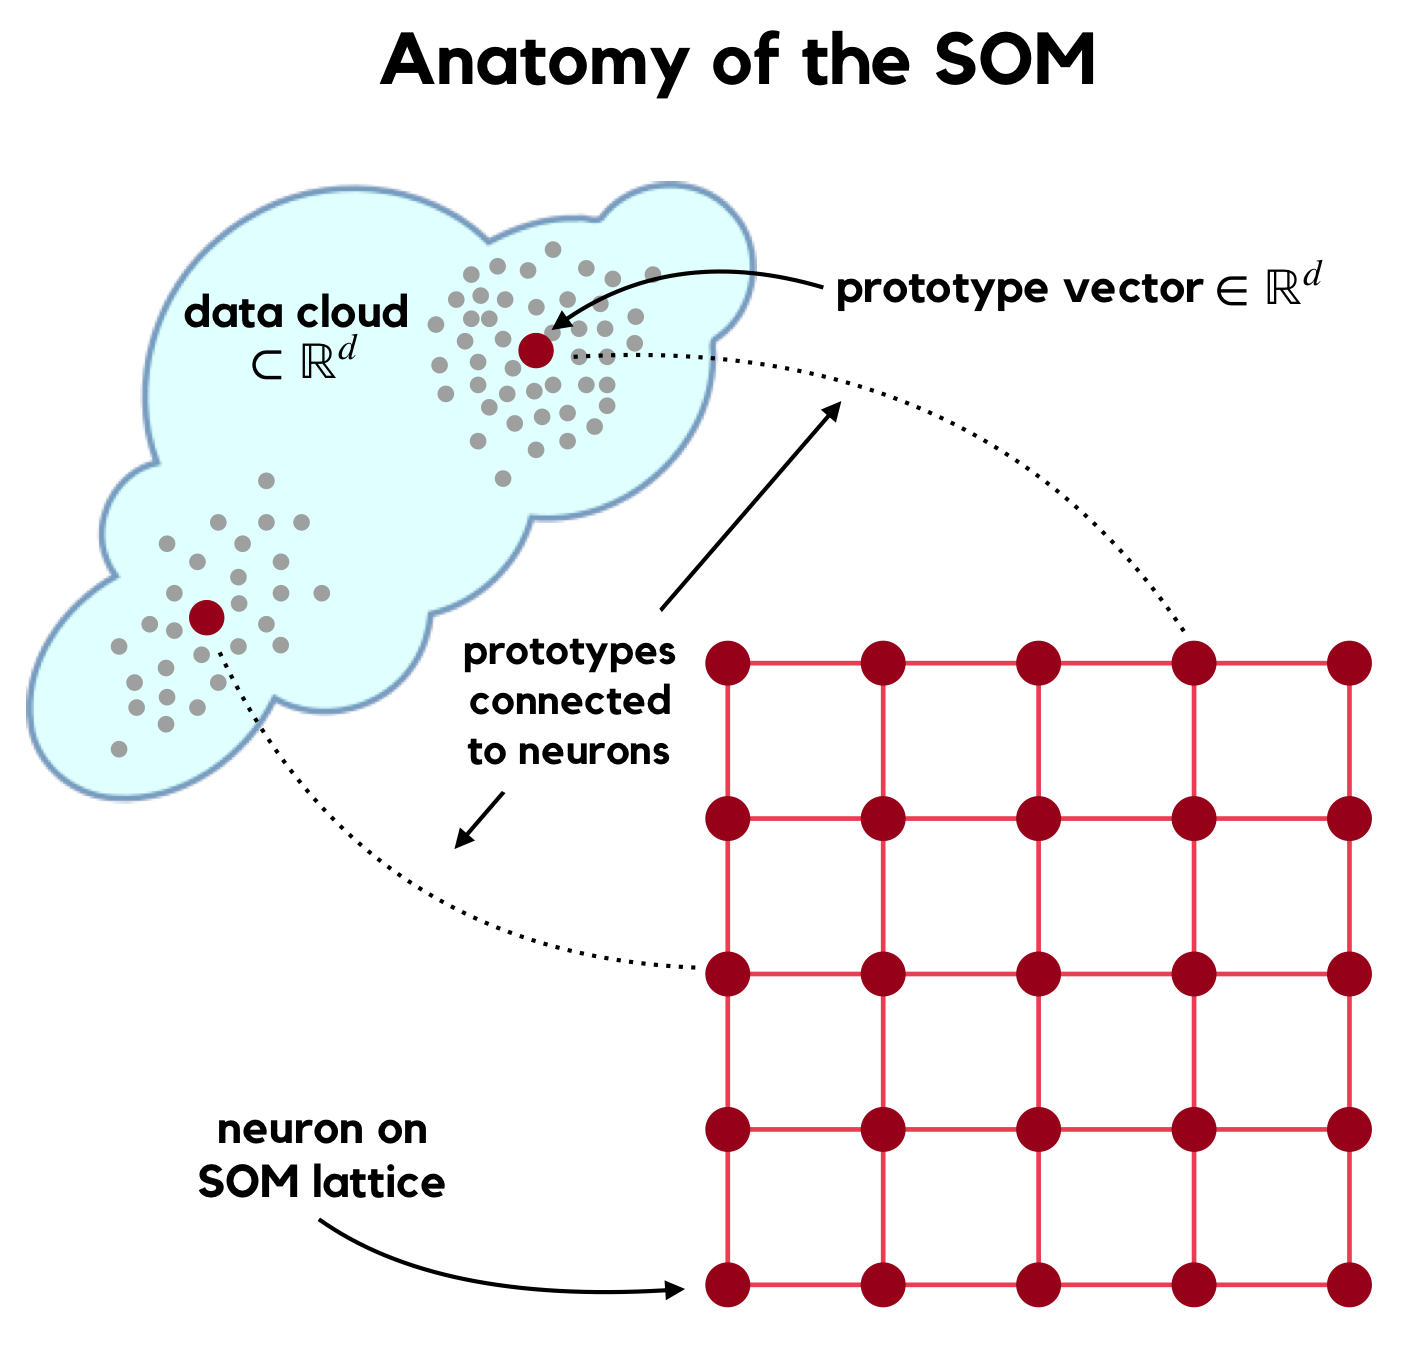
\includegraphics[width=0.7\linewidth]{./figs/som_anatomy} \end{center}

This organization is enforced by cooperative updates to the prototypes during the learning process. At training step \(t\), prototype updates are governed by
\[ w_j^{t} = w_j^{t-1} + \alpha_t \times \eta(j, j^*_t \, | \, \sigma_t) \times (x^t - w_j) \]
where

\begin{itemize}
\tightlist
\item
  \(\alpha_t\) is a learning parameter controlling the amount by which prototypes are allowed to change at step \(t\), which should be annealed over time
\item
  \(x^t \in X\) is a training vector chosen at random for presentation to the network at time \(t\), also called the network \textbf{stimulus} at time \(t\)
\item
  \(\eta\) (the \textbf{neighborhood function}) is a non-increasing function of the lattice distance between neurons \(\nu_j\) and \(\nu_{j^*_t}\), where \(j^*_t\) indexes the prototype closest to the datum \(x^t\). We call this the \textbf{Best Matching Unit} of \(x^t\):
  \[ BMU(x^t) := j^*_t = \arg\min_j \, d_E(w_j, x^t) \]
  where \(d_E\) is standard Euclidean distance.\\
\item
  \(\sigma_t\) is a learning parameter controlling the size of a lattice neighborhood centered about neuron \(\nu_{j^*_t}\); neurons residing in this neighborhood are affected more strongly by the stimulus \(x^t\), with affect inversely proportional to their lattice distance to the BMU.
\end{itemize}

The implication of including the composition of several notions of distance (i.e., in both \(\mathbb{R}^d\) and \(\mathcal{L}\)) in the prototype update rule forms a highly non-linear mapping \(\Phi \, : \, \mathcal{M} \to \mathcal{L}\). \(\Phi\) is \textbf{self-organized}, meaning the relationship between neuron proimities on \(\mathcal{L}\) and prototype proximities in \(\mathcal{M}\) arises organically, without direct optimization of any loss function. SOM Learning is modeled after the organization and compartmentalization of the learning process which occurs in the human brain.

\hypertarget{conscience-som}{%
\subsection{Conscience SOM}\label{conscience-som}}

Kohonen's prototype updates can yield a mapping \(\Phi\) which under-utilizes the quantizer's full codebook (i.e., the set of prototypes \(W\)). Such under-utilizations degrade the richess of the representation of \(\mathcal{M}\) by \(\mathcal{W}\) (and on \(\mathcal{L}\)). To correct this, DeSieno introduced the \textbf{Conscience SOM} (or \textbf{CSOM}, {[}\protect\hyperlink{ref-DeSieno1988}{2}{]}), which introduces a \textbf{bias} to Kohonen's algorithm to achieve a mapping \(\Phi\) with higher entropy. Each prototype possesses its own bias \(b_j^t\) which influences the competitive stage of SOM learning such that CSOM BMU selection at time \(t\) becomes
\[ BMU(x^t) = \arg\min_j \, d_E(w_j, x^t) - b_j^t.\]
The biases \(\{b_j\}\) are formed alongside the prototype vectors during learning via the use of auxiliary quantities \(\{p_j\}\) representing the historical \textbf{win frequencies} of each prototype (i.e, proportion of times a prototype has quantized data during learning). These win frequencies are updated during each learning step by
\[ p_j^t = p_j^{t-1} + \beta_t \times (\mathbb{1}[j = j^*_t] - p_j^{t-1}) \]
yielding a bias
\[ b_j^t = \gamma_t \times \left( \frac{1}{n_W} - p_j^t \right) \]
For maximum-entropy mapping, \(p_j = 1 / n_W\) implying zero bias. The additional learning parameters \(\beta_t\) and \(\gamma_t\) control the degree to which the SOM's ``Conscience'' influences its learning. Like the learning rate \(\alpha_t\) they should both be annealed over time.

A properly trained CSOM can achieve more effective utilization of the SOM's output space {[}\protect\hyperlink{ref-DeSieno1988}{2}{]} which aides (cluster) inference from a trained map. In contrast to Kohonen's cooperative function (\(\eta\)), DeSieno also suggested restricting prototype updates to a very small neighborhood of neurons (e.g., \(\sigma_t = 1\)), which decreases the computational burden of CSOM learning (as compared to Kohonen's SOM). Moreover, as all prototypes are encouraged to participate in the learned representation of \(\mathcal{M}\) the resulting view of the manifold is often richer, providing for more sophisticated cluster extraction tools such as the CADJ matrix.

\hypertarget{the-cadj-matrix}{%
\subsection{The CADJ Matrix}\label{the-cadj-matrix}}

\textbf{CADJ} (or \textbf{C}umulative \textbf{ADJ}acency, {[}\protect\hyperlink{ref-TasdemirMerenyi2009}{3}{]}) is a weighted adjacency matrix of SOM prototypes (or, equivalently, their associated neurons). The edge weights of this \textbf{Topology Representing Network} {[}\protect\hyperlink{ref-MartinetzSchulten1994}{4}{]} are given by
\[ CADJ_{ij} = \# \{x_s \, : \, BMU1(x_s) = i \text{ and } BMU2(x_s) = j \} \]
where BMU1 and BMU2 are the first and second-ranking BMU, respectively. Analysis of the CADJ values reveals the ``seams'' (disconnects) of a learned manifold, which are helpful for discerning cluster structure.

While CADJ can technically be computed using the codebook of \emph{any} vector quantizer as vertices, the SOM's output space \(\mathcal{L}\) provides prime real estate on which to view and analyze this graph, regardless of data dimension \(d\). The \textbf{CONNvis} visiualization {[}\protect\hyperlink{ref-TasdemirMerenyi2009}{3}{]}, derived from the symmetrized \textbf{CONN}ectivity graph,
\[CONN = CADJ + CADJ^T,\]
has been used repeatedly to elicit cluster structure from complex, high-dimensional manifolds with \textbf{no restriction} on cluster size (number of data members), shape (e.g., Gaussianinity), or dimension (low-rank embeddings). These settings are precisely where performance of other clustering routines (e.g., hierarchical methods, k-means, mixture models) deterioriate.

Despite the demonstrated benefits and sophistication of the combination of CSOM manifold learning and subsequent CADJ-based cluster extraction (CITE), neither of these tools are currently publicly available to the machine learning community. SOMDisco rectifies this omission.

\hypertarget{installation}{%
\section{Installation}\label{installation}}

SOMDisco is available for Unix-like systems from github (not CRAN), installable via

\begin{Shaded}
\begin{Highlighting}[]
\NormalTok{devtools}\OperatorTok{::}\KeywordTok{install_github}\NormalTok{(}\StringTok{"somdisco/SOMDisco"}\NormalTok{)}
\end{Highlighting}
\end{Shaded}

Windows users can clone the repository and modify their \texttt{Makevars} files accordingly. The \texttt{DESCRIPTION} file in the package source lists the following 3rd-party R package dependencies:

\begin{verbatim}
Imports: 
    Rcpp (>= 1.0.1), 
    stringr, 
    igraph, 
    dplyr, 
    Rdpack
LinkingTo: Rcpp, RcppArmadillo, RcppParallel
\end{verbatim}

SOM training is made efficient through use of a templated C++ CSOM class. For those who may desire custom or expanded functionality, the class template is implemented in header-only fashion in the \texttt{inst/include} directoy of the package source.

\hypertarget{shgr-example-data}{%
\section{SHGR Example Data}\label{shgr-example-data}}

SOMDisco is packaged alongside an example dataset to showcase its training and analysis capabilities. The SHGRWalk Data (SHGR, for short) are 128 x 128 pixel, 100-dimensional \textbf{S}ynthetic \textbf{H}yperspectral data cubes based on a \textbf{G}aussian \textbf{R}andom \textbf{W}alk across the spectral ``channels''. More information about the data generation and structure of the ``20-class, cov500-4000'' data case included with SOMDisco can be found at the \href{https://somdisco.github.io/SHGRWalk/output/index.html}{SHGRWalk homepage}. Briefly, \texttt{library(SOMDisco)} loads a list named \texttt{SHGR} into the user's R environment with components:

\begin{itemize}
\tightlist
\item
  \texttt{X} the SHGR data, as a data matrix. nrows = 128 x 128 = 16,384 (number of image pixels), ncol = 100 (spectral dimension). Each row contains one spectral ``signature'' from each pixel of the SHGRWalk cube.\\
\item
  \texttt{label} a character vector (length = 16,384) containing labels (``A'' - ``T'') for each pixel of the cube. The order corresponds to the row ordering of \texttt{X}.\\
\item
  \texttt{ctab} a data frame with columns \texttt{label} and \texttt{color} defining the mapping between unique label names (``A'',``B'',\ldots{}``T'') and their associated identifying color
\item
  \texttt{pxl.coords} a 2-column matrix (nrows = 16,384) giving the spatial pixel coordinates ( in \texttt{(row,col)} format) for each spectra in the rows of \texttt{X}
\item
  \texttt{identifier} a string identifying the specific SHGRWalk cube included with SOMDisco (there are others, as explained \href{https://somdisco.github.io/SHGRWalk/output/index.html}{SHGRWalk homepage}).
\end{itemize}

The individual spectra of the pixels comprising each of the 20 unique classes, plotted across the 100 channels, is below:

\begin{center}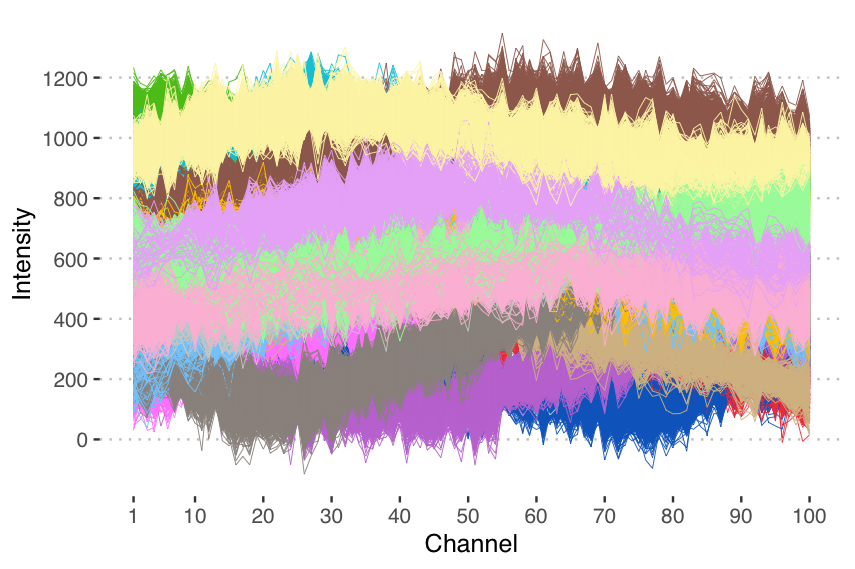
\includegraphics[width=0.7\linewidth]{./figs/SGRW-100d_20class_cov500-4000-spectra} \end{center}

We will utilize the SHGR data in the training and visualization showcases which follow.

\hypertarget{som-initialization}{%
\section{SOM Initialization}\label{som-initialization}}

SOMDisco is built around the internal C++ class \texttt{SOMOBJ}, which is a header-only class (found in the \texttt{/inst/include/} source package) envisioned to be entirely portable for future integration with other SOM-related projects. This section will demonstrate how to interact with the class fields and methods to achieve SOM training (a complete list of the fields and methods of this class exposed to the user by the SOMDisco package can be found with \texttt{?SOM}). All methods are documented in the usual manner, with help functionality available via \texttt{?\textless{}method\_name\textgreater{}}.

To get started with SOM training we must instantiate an empty \texttt{SOM} object, then initialize it with our training data and desired lattice size and topology via the method \texttt{initialize\_SOM}.

\begin{Shaded}
\begin{Highlighting}[]
\KeywordTok{library}\NormalTok{(SOMDisco)}
\NormalTok{mysom =}\StringTok{ }\NormalTok{SOM}\OperatorTok{$}\KeywordTok{new}\NormalTok{()}
\NormalTok{mysom}\OperatorTok{$}\KeywordTok{initialize_SOM}\NormalTok{(SHGR}\OperatorTok{$}\NormalTok{X, }\DecValTok{20}\NormalTok{, }\DecValTok{20}\NormalTok{, }\StringTok{"hex"}\NormalTok{)}
\CommentTok{## Setting lattice quantities}
\CommentTok{## ++ calculating lattice (x,y) coordinates ... done}
\CommentTok{## ++ calculating neuron lattice adjacencies ... done}
\CommentTok{## ++ calculating geodesic lattice distances between neurons ... done}
\CommentTok{## ++ assigning geodesic lattice distances to distlist ... done}
\CommentTok{## ++ calculating lattice tile vertices ... done}
\CommentTok{## ----------------------------------------------------------------}
\CommentTok{## Setting training data}
\CommentTok{## ----------------------------------------------------------------}
\CommentTok{## Setting network ranges}
\CommentTok{## ++ external = [-115.19, 1347.57]}
\CommentTok{## ++ internal = [0.00, 1.00]}
\CommentTok{## ++ change defaults via $set_netrng}
\CommentTok{## ----------------------------------------------------------------}
\CommentTok{## Initializing prototypes to random uniform}
\CommentTok{## ++ to set a particular random seed call set.seed() and then $set_W_runif()}
\CommentTok{## ++ to set to specific values call $set_W()}
\CommentTok{## ----------------------------------------------------------------}
\CommentTok{## Initializing prototype win frequencies to equiprobable}
\CommentTok{## ++ to set to specific values call $set_p(values)}
\CommentTok{## ----------------------------------------------------------------}
\CommentTok{## Setting default learning rates}
\CommentTok{## Storing the annealing schedule as:}
\CommentTok{## t	alpha	beta	gamma	sigma}
\CommentTok{## 16384	0.50	0.05	0.01	3}
\CommentTok{## 81920	0.25	0.03	0.00	2}
\CommentTok{## 163840	0.10	0.01	0.00	1}
\CommentTok{## 409600	0.05	0.01	0.00	1}
\CommentTok{## 1638400	0.01	0.00	0.00	1}
\CommentTok{## ++ change via $get_LRAS and $set_LRAS}
\CommentTok{## ----------------------------------------------------------------}
\end{Highlighting}
\end{Shaded}

The arguments to \texttt{initialize\_SOM} are, in order: the matrix with training data in rows, the desired som lattice width and height (number of neurons along each dimension) and the desired lattice type, which can be either \texttt{"hex"} for hexagonal lattices or \texttt{"grid"} for rectangular lattices. Internally, \texttt{initialize\_SOM} calls several other methods to set required (and internally calculated) quantities related to the SOM lattice, and default parameters for network scaling, prototype initialization, and learning rate annealing. The sample size \texttt{nX} and data dimension \texttt{d} are also stored during this call.

\hypertarget{lattice-quantitites}{%
\subsection{Lattice Quantitites}\label{lattice-quantitites}}

Lattice quantities are fields that generally begin with \texttt{nu\_*} (by our convention, lattice neurons are represented by lower Greek \(\nu\)). These fields can be examined via the \texttt{\$} operator of of the instantiated SOM object:

\begin{Shaded}
\begin{Highlighting}[]
\CommentTok{# The lattice width, height, and type, respectively }
\NormalTok{mysom}\OperatorTok{$}\NormalTok{som_x}
\CommentTok{## [1] 20}
\NormalTok{mysom}\OperatorTok{$}\NormalTok{som_y}
\CommentTok{## [1] 20}
\NormalTok{mysom}\OperatorTok{$}\NormalTok{lattice_type}
\CommentTok{## [1] "hex"}

\CommentTok{# The total number of neurons / prototypes in the SOM. }
\CommentTok{# For hexagonal lattices, this number will be > som_x*som_y}
\NormalTok{mysom}\OperatorTok{$}\NormalTok{nW}
\CommentTok{## [1] 410}

\CommentTok{# The (x,y) coordinates of the neurons on the SOM lattice}
\KeywordTok{str}\NormalTok{(mysom}\OperatorTok{$}\NormalTok{nu_xy)}
\CommentTok{##  num [1:410, 1:2] 1 2 3 4 5 6 7 8 9 10 ...}

\CommentTok{# The (row,col) coordinates of the neurons on the SOM lattice. }
\CommentTok{# These differ from their (x,y) coordinates if lattice_type = 'hex'}
\KeywordTok{str}\NormalTok{(mysom}\OperatorTok{$}\NormalTok{nu_ij)}
\CommentTok{##  num [1:410, 1:2] 1 1 1 1 1 1 1 1 1 1 ...}

\CommentTok{# A binary adjacency matrix representing the topology of neurons on the lattice}
\KeywordTok{str}\NormalTok{(mysom}\OperatorTok{$}\NormalTok{nu_ADJ)}
\CommentTok{##  num [1:410, 1:410] 1 1 0 0 0 0 0 0 0 0 ...}

\CommentTok{# The (x,y) coordinates of the vertices of each lattice tile are stored }
\CommentTok{# in a 3d cube whose slices follow neuron ordering. }
\KeywordTok{str}\NormalTok{(mysom}\OperatorTok{$}\NormalTok{nu_verts)}
\CommentTok{##  num [1:6, 1:2, 1:410] 1.5 1 0.5 0.5 1 ...}
\CommentTok{# e.g., the vertices of the lattice tile centered at the first neuron are: }
\NormalTok{mysom}\OperatorTok{$}\NormalTok{nu_verts[,,}\DecValTok{1}\NormalTok{]}
\CommentTok{##      [,1]      [,2]}
\CommentTok{## [1,]  1.5 1.2886751}
\CommentTok{## [2,]  1.0 1.5773503}
\CommentTok{## [3,]  0.5 1.2886751}
\CommentTok{## [4,]  0.5 0.7113249}
\CommentTok{## [5,]  1.0 0.4226497}
\CommentTok{## [6,]  1.5 0.7113249}

\CommentTok{# A list giving, for all neurons, the indices of others neurons that are }
\CommentTok{# within a certain lattice geodesic distance: }
\KeywordTok{length}\NormalTok{(mysom}\OperatorTok{$}\NormalTok{nu_nhblist)}
\CommentTok{## [1] 410}

\CommentTok{# The vector nu_nhblist[[i]][[j]] contains indices of neurons that are }
\CommentTok{# within geodesic lattice distace j-1 of neuron i. }
\CommentTok{# ex., these neurons are within lattice distance = 1 of the first lattice neuron: }
\NormalTok{mysom}\OperatorTok{$}\NormalTok{nu_nhblist[[}\DecValTok{1}\NormalTok{]][[}\DecValTok{2}\NormalTok{]]}
\CommentTok{## [1]  2 21 22}
\end{Highlighting}
\end{Shaded}

The above quantities are set by the method \texttt{set\_lattice}, but this should rarely need to be called on its own (it is called internally by \texttt{initialize\_SOM}). All containers storing neuron and prototype quantities are ordered such that the first element (or row, or slice, as applicable) corresponds to the neuron at the bottom left of the SOM lattice. Ordering proceeds across the rows of the lattice so that the last element (row, slice) corresponds to the neuron at the top right of the SOM.\\
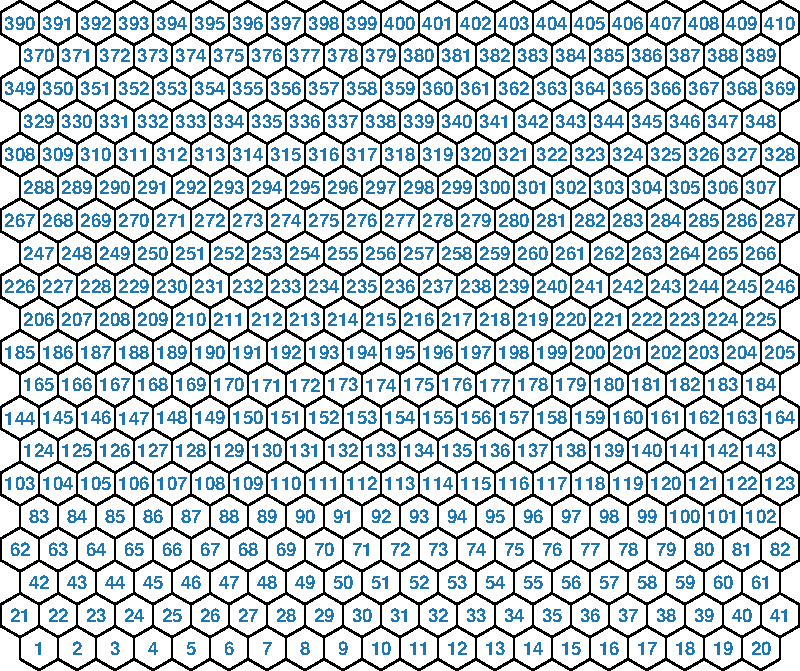
\includegraphics{SOMDisco.README_files/figure-latex/ck-SHGRSOMneuronorder-1.pdf}

This is known as \textbf{neuron ordering}

\hypertarget{network-scaling}{%
\subsection{Network Scaling}\label{network-scaling}}

The \textbf{external network range} is the apparent range of the training data. Internally, the SOM prototypes are stored in an \textbf{internal" network range}, which is necessary to stabilize and accelerate the training process. Both BMU selection and prototype updates are performed in the internal network range. During training, data are mapped (linearly) from the external to internal range for presentation to the network. \texttt{initialize\_SOM} calls the method \texttt{set\_netrng} internally, which sets the min/max of both the external and internal network ranges needed for this mapping to their defaults (which is the apparent dimension-wise range of the training data for the former, and {[}0,1{]} for the latter):

\begin{Shaded}
\begin{Highlighting}[]
\CommentTok{# The default values stored }
\KeywordTok{str}\NormalTok{(mysom}\OperatorTok{$}\NormalTok{netrng_ext_min)}
\CommentTok{##  num [1, 1:100] -115 -115 -115 -115 -115 ...}
\KeywordTok{str}\NormalTok{(mysom}\OperatorTok{$}\NormalTok{netrng_ext_max)}
\CommentTok{##  num [1, 1:100] 1348 1348 1348 1348 1348 ...}
\NormalTok{mysom}\OperatorTok{$}\NormalTok{netrng_int_min}
\CommentTok{## [1] 0}
\NormalTok{mysom}\OperatorTok{$}\NormalTok{netrng_int_max}
\CommentTok{## [1] 1}
\end{Highlighting}
\end{Shaded}

The default network scalings can be changed manually by calling \texttt{set\_netrng} at any point prior to training. See its help for more information.

Once the network ranges are set, data can be mapped from external to internal network ranges (or vice-versa) via the methods \texttt{map\_to\_netrng} and \texttt{map\_from\_netrng}, both of which are parallelized. For example, the entire training set can be mapped to the internal network range via:

\begin{Shaded}
\begin{Highlighting}[]
\KeywordTok{range}\NormalTok{(SHGR}\OperatorTok{$}\NormalTok{X)}
\CommentTok{## [1] -115.1884 1347.5741}
\NormalTok{mapped_training_data =}\StringTok{ }\NormalTok{mysom}\OperatorTok{$}\KeywordTok{map_to_netrng}\NormalTok{(SHGR}\OperatorTok{$}\NormalTok{X)}
\KeywordTok{range}\NormalTok{(mapped_training_data)}
\CommentTok{## [1] 0 1}
\end{Highlighting}
\end{Shaded}

Commonly, the learned SOM prototypes would need to be extracted from the SOM object and returned to external range for direct comparison with the data. This can be achived by:

\begin{Shaded}
\begin{Highlighting}[]
\KeywordTok{range}\NormalTok{(mysom}\OperatorTok{$}\NormalTok{W)}
\CommentTok{## [1] 0.5000002 0.5999968}
\NormalTok{mapped_prototypes =}\StringTok{ }\NormalTok{mysom}\OperatorTok{$}\KeywordTok{map_from_netrng}\NormalTok{(mysom}\OperatorTok{$}\NormalTok{W)}
\KeywordTok{range}\NormalTok{(mapped_prototypes)}
\CommentTok{## [1] 616.1932 762.4644}
\end{Highlighting}
\end{Shaded}

\hypertarget{prototype-initialization}{%
\subsection{Prototype Initialization}\label{prototype-initialization}}

The SOM prototype weights are stored in the rows of the \texttt{nW\ x\ d} prototype matrix \texttt{W}:

\begin{Shaded}
\begin{Highlighting}[]
\KeywordTok{str}\NormalTok{(mysom}\OperatorTok{$}\NormalTok{W)}
\CommentTok{##  num [1:410, 1:100] 0.536 0.569 0.554 0.571 0.554 ...}
\end{Highlighting}
\end{Shaded}

\texttt{initialize\_SOM} calls the method \texttt{set\_W\_runif} automatically, which initializes the prototypes to random uniform values over the middle 10\% of the internal network range. If random seeding of these values is desired for reproducibility, this method should be re-invoked immediately after a call to R's \texttt{set.seed}:

\begin{Shaded}
\begin{Highlighting}[]
\KeywordTok{set.seed}\NormalTok{(}\DecValTok{123}\NormalTok{)}
\NormalTok{mysom}\OperatorTok{$}\KeywordTok{set_W_runif}\NormalTok{()}
\end{Highlighting}
\end{Shaded}

Custom prototype initializations are supported by the general method \texttt{set\_W}, which allows the user to set a desired prototype weight matrix (which must have conforming dimensions: nrows = \texttt{nW} and ncols = \texttt{d}) Here, we set them to random standard normals for demo purposes:

\begin{Shaded}
\begin{Highlighting}[]
\NormalTok{rnorm_protos =}\StringTok{ }\KeywordTok{matrix}\NormalTok{(}\KeywordTok{rnorm}\NormalTok{(mysom}\OperatorTok{$}\NormalTok{nW}\OperatorTok{*}\NormalTok{mysom}\OperatorTok{$}\NormalTok{d), }\DataTypeTok{nrow=}\NormalTok{mysom}\OperatorTok{$}\NormalTok{nW, }\DataTypeTok{ncol=}\NormalTok{mysom}\OperatorTok{$}\NormalTok{d)}
\NormalTok{mysom}\OperatorTok{$}\KeywordTok{set_W}\NormalTok{(rnorm_protos)}
\CommentTok{## Warning in mysom$set_W(rnorm_protos): Input is outside netrng_int. Likely need}
\CommentTok{## to scale to internal network range, then call $set_W()}
\end{Highlighting}
\end{Shaded}

A warning is issued if the prototype matrix contains values outside the internal network range. Custom initializations will likely need to be mapped to internal range prior to setting:

\begin{Shaded}
\begin{Highlighting}[]
\NormalTok{rnorm_protos =}\StringTok{ }\NormalTok{mysom}\OperatorTok{$}\KeywordTok{map_to_netrng}\NormalTok{(rnorm_protos)}
\NormalTok{mysom}\OperatorTok{$}\KeywordTok{set_W}\NormalTok{(rnorm_protos)}
\end{Highlighting}
\end{Shaded}

\hypertarget{win-frequency-initialization}{%
\subsection{Win Frequency Initialization}\label{win-frequency-initialization}}

In addition to the prototypes themselves, DeSieno's CSOM algorithm introduces another learned quantity to facilitate a maximum-entropy SOM mapping: the prototype win frequencies, which are stored in the SOM object in the vector \texttt{p}. The \texttt{p} control the CSOM prototype \texttt{bias}, which affects the competitive stage of BMU selection during SOM training. \texttt{initialize\_SOM} automatically calls the method \texttt{set\_p\_equal}, which sets all prototype win frequences to the value \texttt{1\ /\ nW}. If desired, other initializations can be achieved via the method \texttt{set\_p}, which takes a user-specified vector of win frequencies:

\begin{Shaded}
\begin{Highlighting}[]
\NormalTok{new_p =}\StringTok{ }\KeywordTok{runif}\NormalTok{(mysom}\OperatorTok{$}\NormalTok{nW)}
\NormalTok{mysom}\OperatorTok{$}\KeywordTok{set_p}\NormalTok{(new_p)}
\end{Highlighting}
\end{Shaded}

\hypertarget{learning-rate-initialization}{%
\subsection{Learning Rate Initialization}\label{learning-rate-initialization}}

All CSOM learning rates should be annealed over time. Annealing is controlled by the internally stored data frame \texttt{LRAS} (or Learning Rate Annealing Schedule), which has columns \texttt{t} (setting the cumulative number of training steps over which the given rates are valid), \texttt{alpha} (controlling the strength of the prototype updates), \texttt{beta} (controlling the strength of win frequncy updates), \texttt{gamma} (controlling the influence of the win frequences to the CSOM bias), and \texttt{sigma} (controlling the lattice neighborhood size over which prototype updates occur). \texttt{initialize\_SOM} calls the stand-alone function \texttt{default\_LRAS} by default, which populates an annealing schedule based solely on the training sample size:

\begin{Shaded}
\begin{Highlighting}[]
\KeywordTok{default_LRAS}\NormalTok{(}\DataTypeTok{nX =}\NormalTok{ mysom}\OperatorTok{$}\NormalTok{nX)}
\CommentTok{##         t alpha  beta  gamma sigma}
\CommentTok{## 1   16384  0.50 0.050 0.0050     3}
\CommentTok{## 2   81920  0.25 0.025 0.0025     2}
\CommentTok{## 3  163840  0.10 0.010 0.0010     1}
\CommentTok{## 4  409600  0.05 0.005 0.0005     1}
\CommentTok{## 5 1638400  0.01 0.001 0.0001     1}
\end{Highlighting}
\end{Shaded}

Users can check the current annealing schedule of the SOM object via the method \texttt{get\_LRAS} and set it to new values with \texttt{set\_LRAS}, which takes a data frame of the above form as input. For example, the below will increase the \texttt{alpha} values for all training steps by 10\%:

\begin{Shaded}
\begin{Highlighting}[]
\NormalTok{new_LRAS =}\StringTok{ }\NormalTok{mysom}\OperatorTok{$}\KeywordTok{get_LRAS}\NormalTok{()}
\NormalTok{new_LRAS}\OperatorTok{$}\NormalTok{alpha =}\StringTok{ }\FloatTok{1.10} \OperatorTok{*}\StringTok{ }\NormalTok{new_LRAS}\OperatorTok{$}\NormalTok{alpha }
\NormalTok{mysom}\OperatorTok{$}\KeywordTok{set_LRAS}\NormalTok{(new_LRAS) }
\CommentTok{## Storing the annealing schedule as:}
\CommentTok{## t	alpha	beta	gamma	sigma}
\CommentTok{## 16384	0.55	0.05	0.01	3}
\CommentTok{## 81920	0.28	0.03	0.00	2}
\CommentTok{## 163840	0.11	0.01	0.00	1}
\CommentTok{## 409600	0.06	0.01	0.00	1}
\CommentTok{## 1638400	0.01	0.00	0.00	1}
\end{Highlighting}
\end{Shaded}

At every training step the currently applicable learning rates (based on the SOM's age and the LRAS schedule) are extracted from the LRAS data frame and stored in the following fields by the method \texttt{update\_learning\_rates}:

\begin{Shaded}
\begin{Highlighting}[]
\NormalTok{mysom}\OperatorTok{$}\NormalTok{alpha}
\CommentTok{## [1] 0.55}
\NormalTok{mysom}\OperatorTok{$}\NormalTok{beta}
\CommentTok{## [1] 0.05}
\NormalTok{mysom}\OperatorTok{$}\NormalTok{gamma}
\CommentTok{## [1] 0.005}
\NormalTok{mysom}\OperatorTok{$}\NormalTok{sigma}
\CommentTok{## [1] 3}
\end{Highlighting}
\end{Shaded}

The parameter \texttt{sigma} controls the size of the (lattice) neighborhood (of the prevailing BMU) in which prototypes are updated during each training step. The strength of neighbor updates decreases with their lattice distance from the BMU; the prototypes of any neurons which are greater than \texttt{sigma} away from the BMU will not be updated. The strength of updates to prototype whose neurons are within a \texttt{sigma} lattice radius of the BMU decreases exponentially with this lattice distance. This factor is stored in the SOM object as the parameter \texttt{eta}, which is a vector of length \texttt{sigma\ +\ 1}. The vector element \texttt{eta{[}r{]}} stores a multiplicative coefficient applied to the updates of those prototypes which are distance \texttt{r-1} from the BMU.

\begin{Shaded}
\begin{Highlighting}[]
\NormalTok{mysom}\OperatorTok{$}\NormalTok{eta}
\CommentTok{##           [,1]}
\CommentTok{## [1,] 1.0000000}
\CommentTok{## [2,] 1.0000000}
\CommentTok{## [3,] 0.5994843}
\CommentTok{## [4,] 0.3593814}
\end{Highlighting}
\end{Shaded}

\texttt{eta} is re-calculated any time the effective \texttt{sigma} value is changed (annealed) during training. To enforce the organization of the SOM, \texttt{eta} always = 1 for the BMU and its immediate lattice neighbors. \texttt{eta} is calculated via the method \texttt{calc\_eta}, which should rarely need to be called on its own.

Of note, Kohonen's original prototype algorithm (i.e, without DeSieno's Conscience modification) can be achieved by setting \texttt{beta} and \texttt{gamma} to 0 and annealing a larger \texttt{sigma} radius over time.

\hypertarget{som-learning}{%
\section{SOM Learning}\label{som-learning}}

\hypertarget{network-training}{%
\subsection{Network Training}\label{network-training}}

While several methods exposed to the user participate in SOM training, the main method (and, typically, the only method needing to be called) for SOM training, is \texttt{train\_SOM}. As the \texttt{SOM} class was intetionally designed to not store the training data (to avoid duplicate memory occupation of larger training sets), the matrix of training data must be passed to this method. It should be the same data matrix supplied when calling \texttt{initialize\_SOM} (internal checks will verify this, and return a runtime error if deviations are deteced). The following command performs 100,000 training steps on an SOM object previously initialized to learn the example SHGR data. Status information is automatically printed to the R console.

\begin{Shaded}
\begin{Highlighting}[]
\NormalTok{mysom}\OperatorTok{$}\KeywordTok{train_SOM}\NormalTok{(}\DecValTok{100000}\NormalTok{, SHGR}\OperatorTok{$}\NormalTok{X)}
\CommentTok{## SOM Training:}
\CommentTok{## ++ Reporting every 10000, monitoring every 0steps}
\CommentTok{## 1	2	3	4	5	6	7	8	}
\CommentTok{## 9	10	}
\CommentTok{## End Training (current age = 100000)}
\CommentTok{## ----------------------------------------------------------------}
\CommentTok{## SOM Recall:}
\CommentTok{## ++ finding BMUs of data ... done}
\CommentTok{## ++ building CADJ matrix ... done}
\CommentTok{## ++ setting RF_size ... done}
\CommentTok{## ++ calculating SOM Entropy ... done}
\CommentTok{## ++ populating RF_members ... done}
\CommentTok{## ++ setting lattice fences ... done}
\NormalTok{mysom}\OperatorTok{$}\NormalTok{age }
\CommentTok{## [1] 1e+05}
\end{Highlighting}
\end{Shaded}

Internally, \texttt{train\_SOM} calls the methods \texttt{update\_W} and \texttt{update\_p}, which perform updates to the prototype matrix \texttt{W} and the CSOM win frequencies \texttt{p} at each training step. These methods are exposed to the user, but should not be called separately independently. The \texttt{age} field stores the number of training steps that have been performed during the life of the instantiated SOM object. Additional training can be performed at any time by re-invoking the \texttt{train\_SOM} method. Here, we train the above SOM for another 25,000 steps:

\begin{Shaded}
\begin{Highlighting}[]
\NormalTok{mysom}\OperatorTok{$}\KeywordTok{train_SOM}\NormalTok{(}\DecValTok{25000}\NormalTok{, SHGR}\OperatorTok{$}\NormalTok{X)}
\CommentTok{## SOM Training:}
\CommentTok{## ++ Reporting every 10000, monitoring every 0steps}
\CommentTok{## 1	2	}
\CommentTok{## End Training (current age = 125000)}
\CommentTok{## ----------------------------------------------------------------}
\CommentTok{## SOM Recall:}
\CommentTok{## ++ finding BMUs of data ... done}
\CommentTok{## ++ building CADJ matrix ... done}
\CommentTok{## ++ setting RF_size ... done}
\CommentTok{## ++ calculating SOM Entropy ... done}
\CommentTok{## ++ populating RF_members ... done}
\CommentTok{## ++ setting lattice fences ... done}
\NormalTok{mysom}\OperatorTok{$}\NormalTok{age}
\CommentTok{## [1] 125000}
\end{Highlighting}
\end{Shaded}

Training should proceed until the user is satisfied with the SOM's prototype development and neuron lattice organization. The learned SOM prototype vectors can be extracted from the SOM object via the \texttt{W} field, and should be mapped from internal to external network range if direct comparison to their representative data vectors is desired. Here, we extract the prototypes after the cumulative 125,000 learning steps performed above:

\begin{Shaded}
\begin{Highlighting}[]
\NormalTok{W125k =}\StringTok{ }\NormalTok{mysom}\OperatorTok{$}\NormalTok{W }
\CommentTok{# Return to external network (i.e, data) range }
\NormalTok{W125k =}\StringTok{ }\NormalTok{mysom}\OperatorTok{$}\KeywordTok{map_from_netrng}\NormalTok{(mysom}\OperatorTok{$}\NormalTok{W)}
\end{Highlighting}
\end{Shaded}

Standard online (i.e, not batch) SOM training requires random-order presentation of training data to the network at each training step. A user-specified presentation order for training can be achieved by calling the method \texttt{set\_train\_order} just prior to invoking \texttt{train\_SOM}. \texttt{set\_train\_order} takes a vector of data indices (of length \texttt{nsteps}), which sets the order of the data picked for presentation to the network for the next \texttt{nsteps} training steps. Its input should be 1-based row indices of the training data matrix. Here, we train the above SOM for an additional 10,000 steps where data presentation to the network follows a spefic order:

\begin{Shaded}
\begin{Highlighting}[]
\NormalTok{train_order =}\StringTok{ }\DecValTok{1}\OperatorTok{:}\DecValTok{10000}
\NormalTok{mysom}\OperatorTok{$}\KeywordTok{set_train_order}\NormalTok{(train_order)}
\NormalTok{mysom}\OperatorTok{$}\KeywordTok{train_SOM}\NormalTok{(}\DecValTok{10000}\NormalTok{, SHGR}\OperatorTok{$}\NormalTok{X)}
\CommentTok{## User-specified training order detected. nsteps reset to 10000}
\CommentTok{## SOM Training:}
\CommentTok{## ++ Reporting every 10000, monitoring every 0steps}
\CommentTok{## 1	}
\CommentTok{## End Training (current age = 135000)}
\CommentTok{## ----------------------------------------------------------------}
\CommentTok{## SOM Recall:}
\CommentTok{## ++ finding BMUs of data ... done}
\CommentTok{## ++ building CADJ matrix ... done}
\CommentTok{## ++ setting RF_size ... done}
\CommentTok{## ++ calculating SOM Entropy ... done}
\CommentTok{## ++ populating RF_members ... done}
\CommentTok{## ++ setting lattice fences ... done}
\NormalTok{mysom}\OperatorTok{$}\NormalTok{age}
\CommentTok{## [1] 135000}
\end{Highlighting}
\end{Shaded}

If a specific training order is supplied the number of steps argument to \texttt{train\_SOM} is ignored, and the SOM is trained for \texttt{nsteps\ =\ length(train\_order)}. Setting a training order is uncommon, useful mostly for experimentation and testing.

More commonly a user may wish to retain random presentation of data to the network while also enforcing reproducibility. This can be achieved by calling R's \texttt{set.seed} function just prior to \texttt{train\_SOM}:

\begin{Shaded}
\begin{Highlighting}[]
\KeywordTok{set.seed}\NormalTok{(}\DecValTok{1001}\NormalTok{)}
\NormalTok{mysom}\OperatorTok{$}\KeywordTok{train_SOM}\NormalTok{(}\DecValTok{10000}\NormalTok{, SHGR}\OperatorTok{$}\NormalTok{X)}
\CommentTok{## SOM Training:}
\CommentTok{## ++ Reporting every 10000, monitoring every 0steps}
\CommentTok{## 1	}
\CommentTok{## End Training (current age = 145000)}
\CommentTok{## ----------------------------------------------------------------}
\CommentTok{## SOM Recall:}
\CommentTok{## ++ finding BMUs of data ... done}
\CommentTok{## ++ building CADJ matrix ... done}
\CommentTok{## ++ setting RF_size ... done}
\CommentTok{## ++ calculating SOM Entropy ... done}
\CommentTok{## ++ populating RF_members ... done}
\CommentTok{## ++ setting lattice fences ... done}
\NormalTok{mysom}\OperatorTok{$}\NormalTok{age}
\CommentTok{## [1] 145000}
\end{Highlighting}
\end{Shaded}

\hypertarget{secRecall}{%
\subsection{Network Recall}\label{secRecall}}

After training, the entire training set should be \textbf{recalled} through the SOM, via the method \texttt{recall\_SOM}, which produes additional useful products of SOM learning. A call to \texttt{train\_SOM} automatically ends with a recall, but the recall function is exposed to the user for completeness. Again, it must be given the entire training data matrix (which should match that supplied during \texttt{initialize\_SOM} and \texttt{train\_SOM}):

\begin{Shaded}
\begin{Highlighting}[]
\NormalTok{mysom}\OperatorTok{$}\KeywordTok{recall_SOM}\NormalTok{(SHGR}\OperatorTok{$}\NormalTok{X)}
\CommentTok{## SOM Recall:}
\CommentTok{## ++ finding BMUs of data ... done}
\CommentTok{## ++ building CADJ matrix ... done}
\CommentTok{## ++ setting RF_size ... done}
\CommentTok{## ++ calculating SOM Entropy ... done}
\CommentTok{## ++ populating RF_members ... done}
\CommentTok{## ++ setting lattice fences ... done}
\end{Highlighting}
\end{Shaded}

A recall populates several fields related to the SOM mapping, as described below.

\hypertarget{bmu---som-forwad-map}{%
\subsubsection{BMU - SOM Forwad Map}\label{bmu---som-forwad-map}}

The BMU -- or \textbf{B}est \textbf{M}atching \textbf{U}nit -- of a data vector \(x_s\) is the learned prototype index \(j^*\) satisfying
\[ j^* = \arg\min_{j} \, d_E(w_j, x_s)^2 - b_j\]
where \(d_E(\cdot,\cdot)^2\) is squared Euclidean distance between its vector arguments and \(b_j\) is the learned per-prototype CSOM bias. For a variety of reasons it is useful to calculate and store at least the first and second BMUs (denoted BMU1 and BMU2) for each datum. In general, \(\text{BMU}[k](x_s)\) = the k-th Best Matching Unit (prototype) for the datum indexed by \(s\). The field \texttt{nBMU} controls the number of BMUs computed and stored during recall, and can be set by the method \texttt{set\_nBMU} prior to recall. A default \texttt{nBMU\ =\ 2} is set during a call to \texttt{initialize\_SOM}. Here, we change the number of BMUs to 3, and repeat the recall:

\begin{Shaded}
\begin{Highlighting}[]
\NormalTok{mysom}\OperatorTok{$}\KeywordTok{set_nBMU}\NormalTok{(}\DecValTok{3}\NormalTok{)}
\NormalTok{mysom}\OperatorTok{$}\KeywordTok{recall_SOM}\NormalTok{(SHGR}\OperatorTok{$}\NormalTok{X)}
\CommentTok{## SOM Recall:}
\CommentTok{## ++ finding BMUs of data ... done}
\CommentTok{## ++ building CADJ matrix ... done}
\CommentTok{## ++ setting RF_size ... done}
\CommentTok{## ++ calculating SOM Entropy ... done}
\CommentTok{## ++ populating RF_members ... done}
\CommentTok{## ++ setting lattice fences ... done}
\end{Highlighting}
\end{Shaded}

Note that \texttt{nBMU} must be \(\geq 2\). The BMU information is stored in the field \texttt{BMU}, which is a matrix (nrows = \texttt{nX}, ncols = \texttt{nBMU}) whose (i,j) element gives the j-th BMU index (i.e., the j-th closest prototype) for the datum in row i of the training data matrix. This information can be access via

\begin{Shaded}
\begin{Highlighting}[]
\KeywordTok{head}\NormalTok{(mysom}\OperatorTok{$}\NormalTok{BMU)}
\CommentTok{##      [,1] [,2] [,3]}
\CommentTok{## [1,]    8    9   10}
\CommentTok{## [2,]   10   31   51}
\CommentTok{## [3,]   10    9   31}
\CommentTok{## [4,]   51   31   72}
\CommentTok{## [5,]    9    8   10}
\CommentTok{## [6,]   72   52   51}
\end{Highlighting}
\end{Shaded}

\texttt{BMU} stores the \emph{forward} SOM mapping; that is, the mapping produced from the network \emph{input space} (i.e., data space, or \(\mathbb{R}^d\)), to the network \emph{output space} (i.e, the neurons on the SOM lattice).

\hypertarget{rf_members---som-reverse-map}{%
\subsubsection{RF\_members - SOM Reverse Map}\label{rf_members---som-reverse-map}}

The \emph{reverse} SOM mapping is also stored during \texttt{recall\_SOM} in the field \texttt{RF\_members}, where the prefix ``RF'' stands for \textbf{R}eceptive \textbf{F}ield . This field identifies the mapping from SOM \emph{output space} to \emph{input space}, represented by a list of \texttt{length\ =\ nW} whose i-th entry is a vector of the 1-based data indices (rows of the training data matrix) for whom prototype i is BMU1. For example, the data indices in the Receptive Field of prototype index 10 can be accessed via

\begin{Shaded}
\begin{Highlighting}[]
\NormalTok{mysom}\OperatorTok{$}\NormalTok{RF_members[[}\DecValTok{10}\NormalTok{]]}
\CommentTok{##   [1]    2    3   11  150  265  269  278  283  386  391  397  403  411  414  514}
\CommentTok{##  [16]  518  523  531  542  644  647  649  650  658  668  670  671  770  776  792}
\CommentTok{##  [31]  797  900  902  915 1157 1162 1163 1170 1171 1174 1175 1177 1178 1281 1295}
\CommentTok{##  [46] 1303 1412 1425 1432 1545 1550 1551 1553 1568 1665 1666 1675 1684 1690 1692}
\CommentTok{##  [61] 1696 1793 1800 1813 1815 1818 1929 1931 1935 1937 1938 1941 1947 2063 2185}
\CommentTok{##  [76] 2190 2196 2308 2314 2322 2323 2433 2435 2444 2445 2570 2574 2592 2690 2693}
\CommentTok{##  [91] 2699 2826 2952 2961 2964 2966 2970 2976 3074 3076 3077 3079 3098 3099 3205}
\CommentTok{## [106] 3225 3228 3232 3345 3347 3349 3458 3472 3475 3483 3484 3589 3599 3601 3603}
\CommentTok{## [121] 3615 3719 3725 3727 3733 3858 3860 3866 3982 3983 3996}
\end{Highlighting}
\end{Shaded}

While CSOM attempts an equiprobable quantization of the entire training set by the prototypes, some prototypes will have empty Receptive Fields (meaning they do not quantize any data). If prototype \(j\)'s Receptive Field is empty, then \texttt{RF\_members{[}{[}j{]}{]}} is an empty vector (of length = 0).

\hypertarget{rf_size}{%
\subsubsection{RF\_size}\label{rf_size}}

The size of a prototype's receptive field is the number of datum it quantizes (the size of \texttt{RF\_members{[}{[}j{]}{]}}). This information is stored in the field \texttt{RF\_size}, accessible via

\begin{Shaded}
\begin{Highlighting}[]
\KeywordTok{head}\NormalTok{(mysom}\OperatorTok{$}\NormalTok{RF_size, }\DataTypeTok{n=}\DecValTok{10}\NormalTok{)}
\CommentTok{##       [,1]}
\CommentTok{##  [1,]   83}
\CommentTok{##  [2,]   50}
\CommentTok{##  [3,]   81}
\CommentTok{##  [4,]    0}
\CommentTok{##  [5,]   30}
\CommentTok{##  [6,]  141}
\CommentTok{##  [7,]    0}
\CommentTok{##  [8,]   62}
\CommentTok{##  [9,]   59}
\CommentTok{## [10,]  131}
\end{Highlighting}
\end{Shaded}

Note that \texttt{sum(RF\_size)\ =\ nX} (all data are represented by \emph{some} prototype, hence the sum of the sizes of all prototype's Receptive Fields must equal the training sample size). \texttt{RF\_size} is useful both in analysis and visualization, as large deviations in Receptive Field size between neighboring lattice neurons can indicate cluster boundaries or pattern transitions on the SOM.

\hypertarget{quantization-error}{%
\subsubsection{Quantization Error}\label{quantization-error}}

The distance between a datum \(x_s\) and its BMU \(j^*\) represents the Quantization Error induced by quantizing \(x_s\) by \(w_{j^*}\). These (squared) distances are computed during BMU selection and stored in the field \texttt{SQE}, which is a vector (length = \texttt{nX}) of the \textbf{S}quared \textbf{Q}uantization \textbf{E}rror arising from the SOM mapping, accessible via

\begin{Shaded}
\begin{Highlighting}[]
\KeywordTok{str}\NormalTok{(mysom}\OperatorTok{$}\NormalTok{SQE)}
\CommentTok{##  num [1:16384, 1] 0.0927 0.0843 0.0604 0.1515 0.1142 ...}
\end{Highlighting}
\end{Shaded}

\hypertarget{entropy}{%
\subsubsection{Entropy}\label{entropy}}

The normalized entropy of the forward SOM mapping is stored in the field \texttt{Entropy}. The discrete representation of the manifold from which the training data was drawn drives this entropy calculation, defined as
\[ \text{Entropy} = \frac{1}{\log_2(nW)} \sum\limits_{j=1}^{nW} \frac{\text{RF\_size}_j}{nX} \times \log_2\left( \frac{\text{RF\_size}_j}{nX} \right)\]
The above is normalized so that \(0 \leq \text{Entropy} \leq 1\), and \(\text{Entropy} = 1\) means all prototypes quantize the same number of training data vectors. The normalized entropy of the current SOM mapping is accessible via

\begin{Shaded}
\begin{Highlighting}[]
\NormalTok{mysom}\OperatorTok{$}\NormalTok{Entropy}
\CommentTok{## [1] 0.9461503}
\end{Highlighting}
\end{Shaded}

\hypertarget{u-matrix-fences}{%
\subsubsection{U-Matrix Fences}\label{u-matrix-fences}}

The U-Matrix {[}\protect\hyperlink{ref-UMatrix}{5}{]} and mU-Matrix {[}\protect\hyperlink{ref-MerenyiJainVillmann}{6}{]} visualizations require computing distances between all prototypes whose neurons are lattice-adjacenct. This is done automatically during \texttt{recall\_SOM} using the learned prototype vectors in \texttt{W} and the lattice adjacency matrix \texttt{nu\_ADJ}. The results are stored in the field \texttt{fences}, which is a data frame whose rows represent individual fence information of the form

\begin{Shaded}
\begin{Highlighting}[]
\KeywordTok{head}\NormalTok{(mysom}\OperatorTok{$}\NormalTok{fences)}
\CommentTok{##   i j  x0        y0  x1       y1       value}
\CommentTok{## 1 1 2 1.5 0.7113249 1.5 1.288675 0.011281060}
\CommentTok{## 2 2 3 2.5 0.7113249 2.5 1.288675 0.011196895}
\CommentTok{## 3 3 4 3.5 0.7113249 3.5 1.288675 2.898032735}
\CommentTok{## 4 4 5 4.5 0.7113249 4.5 1.288675 0.432551597}
\CommentTok{## 5 5 6 5.5 0.7113249 5.5 1.288675 0.003857276}
\CommentTok{## 6 6 7 6.5 0.7113249 6.5 1.288675 2.707473984}
\end{Highlighting}
\end{Shaded}

The columns \texttt{i} and \texttt{j} give the two neurons (their indices) which are separated by the fence in each row; the columns \texttt{x0}, \texttt{y0}, \texttt{x1}, \texttt{y1} give the \((x,y)\) coordinates of the endpoints of each fence (as visualized on the lattice); the \texttt{value} column stores the squared Euclidean distance between prototypes \(W_i\) and \(W_j\). This data frame can be populated by a separate call to method \texttt{set\_lattice\_fences} but this is generally unnecessary as it is done automatically in \texttt{recall\_SOM}.

\hypertarget{cadj-conn}{%
\subsubsection{CADJ \& CONN}\label{cadj-conn}}

The CADJ matrix {[}\protect\hyperlink{ref-TasdemirMerenyi2009}{3}{]} is a weighted adjacency matrix of SOM prototypes (neurons) whose \((i,j)\) elements are defined by
\[ \text{CADJ}_{ij} = \#\{x_s \, : \, BMU1(x_s)=i \text{ and } BMU2(x_s)=j \}. \]
Thus, the matrix entries count the number of data vectors for whom prototype \(i\) is first-BMU and \(j\) is second-BMU. This matrix, when visualized on the SOM lattice, is useful for inferring the topological (dis-)connectivities of the manifold underlying the data \(X\) in \(\mathbb{R}^d\). It is accessible via the \texttt{CADJ} field of a recalled SOM object:

\begin{Shaded}
\begin{Highlighting}[]
\KeywordTok{str}\NormalTok{(mysom}\OperatorTok{$}\NormalTok{CADJ)}
\CommentTok{##  num [1:410, 1:410] 0 13 0 0 0 0 0 0 0 0 ...}
\end{Highlighting}
\end{Shaded}

Its symmetrized version, called CONN, is also accessible. Since \(CONN = CADJ + CADJ^T\) it is never stored in the SOM object, merely recreated upon demand. As such, CONN is accessible by calling the \texttt{CONN} \emph{method} (not field):

\begin{Shaded}
\begin{Highlighting}[]
\KeywordTok{str}\NormalTok{(mysom}\OperatorTok{$}\KeywordTok{CONN}\NormalTok{())}
\CommentTok{##  num [1:410, 1:410] 0 35 0 0 0 0 0 0 0 0 ...}
\end{Highlighting}
\end{Shaded}

\hypertarget{recalling-labeled-data}{%
\subsection{Recalling Labeled Data}\label{recalling-labeled-data}}

If the training data possesses associated discrete labels (such as cluster or class membership) it is often helpful to propagate these labels through the forward SOM mapping (which is known as ``labeling the prototypes'') to assess the organization of the lattice, determine the quality of the labels, or both. \emph{If} the labels are meaningful (such that they define genuinely distinct data classes or clusters), and \emph{if} SOM learning is adequate (i.e., performed correctly over enough training steps), then one expects an organization of prototype labels on the lattice. Propagation of data labels through the SOM is achieved by the method \texttt{set\_RF\_label}, which takes a vector of character labels, with one entry for every row of the training data \(X\). Using the labels of the example SHGR data stored in \texttt{SHGR\$label}, label propagation is performed via

\begin{Shaded}
\begin{Highlighting}[]
\NormalTok{mysom}\OperatorTok{$}\KeywordTok{set_RF_label}\NormalTok{(SHGR}\OperatorTok{$}\NormalTok{label)}
\end{Highlighting}
\end{Shaded}

The above method sets two different fields of the \texttt{SOM} object:

\begin{itemize}
\tightlist
\item
  \texttt{RF\_label\_dist} is a list (length = \texttt{nW}) of named integer vectors representing the distribution (contingency count) of the labels mapped to each prototype's Receptive Field. The \texttt{names} attribute of the vector stores the label whereas the vector elements store the associated count. Obviously, the sum of this vector equals the corresponding \texttt{RF\_size}.
\item
  \texttt{RF\_label} is a character vector (length = \texttt{nW}) of the ``winning label'' in each RF, which is the plurality winning label of each RF's distribution (found in \texttt{RF\_label\_dist}). The plurality winner for a RF is the label with highest contingency count.
\end{itemize}

For example, the table of label counts and the plurality label of the first prototype in the SHGR SOM are:

\begin{Shaded}
\begin{Highlighting}[]
\NormalTok{mysom}\OperatorTok{$}\NormalTok{RF_label_dist[[}\DecValTok{1}\NormalTok{]]}
\CommentTok{##  J }
\CommentTok{## 83}
\NormalTok{mysom}\OperatorTok{$}\NormalTok{RF_label[}\DecValTok{1}\NormalTok{]}
\CommentTok{## [1] "J"}
\end{Highlighting}
\end{Shaded}

These fields are primarily useful for label visualization, discussed in Section \ref{secVis}? The SOM object must be trained (and recalled) prior to calling \texttt{set\_RF\_label}.

\hypertarget{monitoring-learning}{%
\subsection{Monitoring Learning}\label{monitoring-learning}}

While there is no universal criteria to determine the number of training steps required for an SOM to properly learn and represent arbitrary manifolds there are a few rules of thumb which help assess the suitability of such learning. During training the SOM undergoes two phases: the initial \emph{organization} phase aligns the neurons on the lattice such that the resulting mapping is \emph{topology preserving} (which usually occurs relatively quickly) while the \emph{convergence} phase further develops the prototypes to best represent the input data (which can take quite some time, depending on the learning parameters used). As a vector quantizer, the SOM should be trained until it is stable and represents the input data reasonably well. To assess these criteria snapshots of the SOM mapping can be taken at various points in (training) time and compared to each other to determine a suitable point at which to terminate training.

The first criterion above is represented by the QSI -- or \textbf{Q}uantization \textbf{S}tability \textbf{I}ndex -- which, at any snapshot time step \(\tau\), reports the proportion of data vectors whose BMUs have changed since the previous snapshot at time \(\tau - 1\). That is,
\[ QSI(\tau) = \frac{1}{nX} \sum\limits_{s=1}^{nX} \#\{ BMU_{\tau-1}(x_s) \, \neq \, BMU_{\tau}(x_s) \}\]
As proper learning proceeds over time we expect \(QSI(\tau) \to 0\). The second criterion above is captured by the overall RMSQE -- or \textbf{R}oot \textbf{M}ean \textbf{S}quare \textbf{Q}uantization \textbf{E}rror -- of the mapping, which is the root average of the \texttt{SQE} of each data vector (as explained in Section \ref{secRecall}). At snapshot time \(\tau\) this is
\[ RMSQE(\tau) = \sqrt{ \frac{1}{nX} \sum\limits_{s=1}^{nX} d_E^2(x_s, w_{j^*_{\tau}}) } \]
where \(d_E^2(\cdot,\cdot)\) is squared Euclidean distance and the notation \(w_{j^*_{\tau}}\) denotes the prevailing prototype BMU of data vector \(x_s\) at snapshot time \(\tau\).Conscience-SOM learning provides a third suitable metric to assess the quality of SOM training. Designed to produce maximum-entropy SOM mappings, a CSOM should be trained until its Entropy (section \ref{secRecall}) is maximal, or at least has stabilized at some near-maximal plateau.

Monitoring of these quantities can be activated prior to SOM training via the method \texttt{set\_monitoring\_freq}, which takes as argument the \emph{incremental} number of steps between monitoring snapshots and stores this argument in the field \texttt{mtr\_freq}. By default, \texttt{initialize\_SOM} sets \texttt{mtr\_freq\ =\ 0} which means no monitoring is performed. Here, we reset the SHGR SOM and repeat training for 100,000 steps with monitoring activated at every 10,000 steps:

\begin{Shaded}
\begin{Highlighting}[]
\CommentTok{# Initialize the SOM }
\NormalTok{mysom =}\StringTok{ }\NormalTok{SOM}\OperatorTok{$}\KeywordTok{new}\NormalTok{()}
\NormalTok{mysom}\OperatorTok{$}\KeywordTok{initialize_SOM}\NormalTok{(SHGR}\OperatorTok{$}\NormalTok{X, }\DecValTok{20}\NormalTok{, }\DecValTok{20}\NormalTok{, }\StringTok{"hex"}\NormalTok{)}
\CommentTok{## Setting lattice quantities}
\CommentTok{## ++ calculating lattice (x,y) coordinates ... done}
\CommentTok{## ++ calculating neuron lattice adjacencies ... done}
\CommentTok{## ++ calculating geodesic lattice distances between neurons ... done}
\CommentTok{## ++ assigning geodesic lattice distances to distlist ... done}
\CommentTok{## ++ calculating lattice tile vertices ... done}
\CommentTok{## ----------------------------------------------------------------}
\CommentTok{## Setting training data}
\CommentTok{## ----------------------------------------------------------------}
\CommentTok{## Setting network ranges}
\CommentTok{## ++ external = [-115.19, 1347.57]}
\CommentTok{## ++ internal = [0.00, 1.00]}
\CommentTok{## ++ change defaults via $set_netrng}
\CommentTok{## ----------------------------------------------------------------}
\CommentTok{## Initializing prototypes to random uniform}
\CommentTok{## ++ to set a particular random seed call set.seed() and then $set_W_runif()}
\CommentTok{## ++ to set to specific values call $set_W()}
\CommentTok{## ----------------------------------------------------------------}
\CommentTok{## Initializing prototype win frequencies to equiprobable}
\CommentTok{## ++ to set to specific values call $set_p(values)}
\CommentTok{## ----------------------------------------------------------------}
\CommentTok{## Setting default learning rates}
\CommentTok{## Storing the annealing schedule as:}
\CommentTok{## t	alpha	beta	gamma	sigma}
\CommentTok{## 16384	0.50	0.05	0.01	3}
\CommentTok{## 81920	0.25	0.03	0.00	2}
\CommentTok{## 163840	0.10	0.01	0.00	1}
\CommentTok{## 409600	0.05	0.01	0.00	1}
\CommentTok{## 1638400	0.01	0.00	0.00	1}
\CommentTok{## ++ change via $get_LRAS and $set_LRAS}
\CommentTok{## ----------------------------------------------------------------}

\CommentTok{# Set the desired snapshot window }
\NormalTok{mysom}\OperatorTok{$}\KeywordTok{set_monitoring_freq}\NormalTok{(}\DecValTok{10000}\NormalTok{)}
\NormalTok{mysom}\OperatorTok{$}\NormalTok{mtr_freq}
\CommentTok{## [1] 10000}

\CommentTok{# Train }
\NormalTok{mysom}\OperatorTok{$}\KeywordTok{train_SOM}\NormalTok{(}\DecValTok{100000}\NormalTok{, SHGR}\OperatorTok{$}\NormalTok{X)}
\CommentTok{## SOM Training:}
\CommentTok{## ++ Reporting every 10000, monitoring every 10000steps}
\CommentTok{## 1	2	3	4	5	6	7	8	}
\CommentTok{## 9	10	}
\CommentTok{## End Training (current age = 100000)}
\CommentTok{## ----------------------------------------------------------------}
\CommentTok{## SOM Recall:}
\CommentTok{## ++ finding BMUs of data ... done}
\CommentTok{## ++ building CADJ matrix ... done}
\CommentTok{## ++ setting RF_size ... done}
\CommentTok{## ++ calculating SOM Entropy ... done}
\CommentTok{## ++ populating RF_members ... done}
\CommentTok{## ++ setting lattice fences ... done}
\end{Highlighting}
\end{Shaded}

The status message displayed during training will indicate the monitoring frequency. After training, the monitored quantities can be extracted via:

\begin{Shaded}
\begin{Highlighting}[]
\CommentTok{# The training ages at which snapshots were taken}
\KeywordTok{head}\NormalTok{(mysom}\OperatorTok{$}\NormalTok{mtr_age)}
\CommentTok{## [1] 10000 20000 30000 40000 50000 60000}

\CommentTok{# The QSI at each monitoring snapshot. }
\CommentTok{# By convention, the first QSI is NA because it compares two snapshots}
\KeywordTok{head}\NormalTok{(mysom}\OperatorTok{$}\NormalTok{mtr_QSI)}
\CommentTok{## [1]        NA 0.9737549 0.8994141 0.9227905 0.9181519 0.8999023}

\CommentTok{# The RMSQE at each monitoring snapshot}
\KeywordTok{head}\NormalTok{(mysom}\OperatorTok{$}\NormalTok{mtr_RMSQE)}
\CommentTok{## [1] 0.3396971 0.3175579 0.3162862 0.3179908 0.3151195 0.3162051}

\CommentTok{# The Entropies at each monitoring snapshot}
\KeywordTok{head}\NormalTok{(mysom}\OperatorTok{$}\NormalTok{mtr_Entropy)}
\CommentTok{## [1] 0.8158475 0.8925877 0.8910236 0.8914353 0.8930978 0.8882450}
\end{Highlighting}
\end{Shaded}

These quantities can be visualized as time series for user analysis (see Section \ref{secVis}).

\textbf{Note:} Most of the recall quantities described above will be computed at each monitoring snapshot. Care should be taken to set \texttt{mtr\_freq} appropriately: it should be small enough to capture meaningful trends in the monitored quantities but also large enough to not incur substantial increase in training time, as the recall is a computationally expensive part of SOM learning.

\hypertarget{parallel-processing}{%
\subsection{Parallel Processing}\label{parallel-processing}}

SOMDisco's parallel implementation is supported by \href{https://cran.r-project.org/web/packages/RcppParallel/index.html}{RcppParallel}. By default, \texttt{initialize\_SOM} activates parallel computation of all possible quantities involved in SOM training and recall. For online (sequential) SOM training, this includes BMU selection and prototype updates at each training step. Most recall quantities can be processed in parallel.

The \texttt{parallel} field of an instantiated SOM object controls whether computation is performed in parallel. To disable parallel processing, the \texttt{set\_parallel} method can be used to set \texttt{parallel\ =\ FALSE}:

\begin{Shaded}
\begin{Highlighting}[]
\CommentTok{# View existint parallel status }
\NormalTok{mysom}\OperatorTok{$}\NormalTok{parallel}
\CommentTok{## [1] TRUE}

\CommentTok{# To disable }
\NormalTok{mysom}\OperatorTok{$}\KeywordTok{set_parallel}\NormalTok{(}\OtherTok{FALSE}\NormalTok{)}

\CommentTok{# Check }
\NormalTok{mysom}\OperatorTok{$}\NormalTok{parallel }
\CommentTok{## [1] FALSE}
\end{Highlighting}
\end{Shaded}

Machine specific threading can be controlled via RcppParallel functions. To control the number of threads made available for parallel processing, see \texttt{?RcppParallel::defaultNumThreads} and \texttt{?RcppParallel::setThreadOptions}. When SOMDisco is loaded (via \texttt{library(SOMDisco)}), the following command is issued to the current R environment, which reserves one thread from processing for other uses:

\begin{Shaded}
\begin{Highlighting}[]
\NormalTok{RcppParallel}\OperatorTok{::}\KeywordTok{setThreadOptions}\NormalTok{(}\DataTypeTok{numThreads =}\NormalTok{ RcppParallel}\OperatorTok{::}\KeywordTok{defaultNumThreads}\NormalTok{() }\OperatorTok{-}\StringTok{ }\DecValTok{1}\NormalTok{)}
\end{Highlighting}
\end{Shaded}

\hypertarget{saving-loading}{%
\subsection{Saving \& Loading}\label{saving-loading}}

Trained SOM objects can be saved to disk for future access via the \texttt{save} method. This method requires a user-specified file name and \textbf{must have extension \texttt{.som}}.

\begin{Shaded}
\begin{Highlighting}[]
\CommentTok{# Save method, filename must have .som extension }
\NormalTok{mysom}\OperatorTok{$}\KeywordTok{save}\NormalTok{(}\StringTok{"mysom.som"}\NormalTok{)}
\end{Highlighting}
\end{Shaded}

While the file has extension \texttt{.som} it is saved in R's binary \texttt{.rds} format as a list. R's \texttt{load} command \emph{can} be used to return this list to the user's environment in a new R session, but the pointers to the C++ object are destroyed on exit of the first session. The \texttt{load} method will properly restore a trained and previously saved SOM object to memory. Once loaded all object methods are available. For example, we can load the previously saved SOM and continue training (with the same SHGR data):

\begin{Shaded}
\begin{Highlighting}[]
\CommentTok{# Load the prevoiusly saved .som file }
\NormalTok{mysom2 =}\StringTok{ }\NormalTok{SOMDisco}\OperatorTok{::}\NormalTok{SOM}\OperatorTok{$}\KeywordTok{new}\NormalTok{() }
\NormalTok{mysom2}\OperatorTok{$}\KeywordTok{load}\NormalTok{(}\StringTok{"mysom.som"}\NormalTok{)}
\CommentTok{## ++ calculating lattice (x,y) coordinates ... done}
\CommentTok{## ++ calculating neuron lattice adjacencies ... done}
\CommentTok{## ++ calculating geodesic lattice distances between neurons ... done}
\CommentTok{## ++ assigning geodesic lattice distances to distlist ... done}
\CommentTok{## ++ calculating lattice tile vertices ... done}
\CommentTok{## Storing the annealing schedule as:}
\CommentTok{## t	alpha	beta	gamma	sigma}
\CommentTok{## 16384	0.50	0.05	0.01	3}
\CommentTok{## 81920	0.25	0.03	0.00	2}
\CommentTok{## 163840	0.10	0.01	0.00	1}
\CommentTok{## 409600	0.05	0.01	0.00	1}
\CommentTok{## 1638400	0.01	0.00	0.00	1}

\CommentTok{# Check that it is the same}
\NormalTok{mysom2}\OperatorTok{$}\NormalTok{age }
\CommentTok{## [1] 1e+05}

\CommentTok{# Re-train for another 10000 steps }
\NormalTok{mysom2}\OperatorTok{$}\KeywordTok{train_SOM}\NormalTok{(}\DecValTok{10000}\NormalTok{, SHGR}\OperatorTok{$}\NormalTok{X)}
\CommentTok{## SOM Training:}
\CommentTok{## ++ Reporting every 10000, monitoring every 10000steps}
\CommentTok{## 1	}
\CommentTok{## End Training (current age = 110000)}
\CommentTok{## ----------------------------------------------------------------}
\CommentTok{## SOM Recall:}
\CommentTok{## ++ finding BMUs of data ... done}
\CommentTok{## ++ building CADJ matrix ... done}
\CommentTok{## ++ setting RF_size ... done}
\CommentTok{## ++ calculating SOM Entropy ... done}
\CommentTok{## ++ populating RF_members ... done}
\CommentTok{## ++ setting lattice fences ... done}
\end{Highlighting}
\end{Shaded}

\hypertarget{secVis}{%
\section{A Complete Example with Visualizations}\label{secVis}}

In this section we exercise a typical standard use of SOMDisco and demonstrate how the supporting SOM visualization functions can be used to aid inference and cluster extraction from a trained SOM. The SOM is unique among vector quantizers in that it possesses a predefined output topology (typically 2-d, as is our setting) which can be harnessed to compactly express the information learned by an SOM for easy inspection.

For speed, all custom SOM visualizations are predicated on R's \texttt{base::plot} functionality (vs., e.g., ggplot). Each of the visualization functions demonstrated in this section are intended to work together (via plot layering) to allow simultaneous representation of multiple learned SOM quantities. Many customization options exist for the visualization functions; their individual help menus explain this optionality.

\begin{Shaded}
\begin{Highlighting}[]
\KeywordTok{library}\NormalTok{(SOMDisco)}
\KeywordTok{library}\NormalTok{(TopoRNet)}
\end{Highlighting}
\end{Shaded}

To begin, we will setup a new SOM object for SHGR training:

\begin{Shaded}
\begin{Highlighting}[]
\CommentTok{# Initialize a 20x20 SOM with hexagonal lattice }
\NormalTok{mysom =}\StringTok{ }\NormalTok{SOM}\OperatorTok{$}\KeywordTok{new}\NormalTok{() }
\NormalTok{mysom}\OperatorTok{$}\KeywordTok{initialize_SOM}\NormalTok{(SHGR}\OperatorTok{$}\NormalTok{X, }\DecValTok{20}\NormalTok{, }\DecValTok{20}\NormalTok{, }\StringTok{"hex"}\NormalTok{)}
\CommentTok{## Setting lattice quantities}
\CommentTok{## ++ calculating lattice (x,y) coordinates ... done}
\CommentTok{## ++ calculating neuron lattice adjacencies ... done}
\CommentTok{## ++ calculating geodesic lattice distances between neurons ... done}
\CommentTok{## ++ assigning geodesic lattice distances to distlist ... done}
\CommentTok{## ++ calculating lattice tile vertices ... done}
\CommentTok{## ----------------------------------------------------------------}
\CommentTok{## Setting training data}
\CommentTok{## ----------------------------------------------------------------}
\CommentTok{## Setting network ranges}
\CommentTok{## ++ external = [-115.19, 1347.57]}
\CommentTok{## ++ internal = [0.00, 1.00]}
\CommentTok{## ++ change defaults via $set_netrng}
\CommentTok{## ----------------------------------------------------------------}
\CommentTok{## Initializing prototypes to random uniform}
\CommentTok{## ++ to set a particular random seed call set.seed() and then $set_W_runif()}
\CommentTok{## ++ to set to specific values call $set_W()}
\CommentTok{## ----------------------------------------------------------------}
\CommentTok{## Initializing prototype win frequencies to equiprobable}
\CommentTok{## ++ to set to specific values call $set_p(values)}
\CommentTok{## ----------------------------------------------------------------}
\CommentTok{## Setting default learning rates}
\CommentTok{## Storing the annealing schedule as:}
\CommentTok{## t	alpha	beta	gamma	sigma}
\CommentTok{## 16384	0.50	0.05	0.01	3}
\CommentTok{## 81920	0.25	0.03	0.00	2}
\CommentTok{## 163840	0.10	0.01	0.00	1}
\CommentTok{## 409600	0.05	0.01	0.00	1}
\CommentTok{## 1638400	0.01	0.00	0.00	1}
\CommentTok{## ++ change via $get_LRAS and $set_LRAS}
\CommentTok{## ----------------------------------------------------------------}

\CommentTok{# For reproducibility, re-initialize the prototypes with a given seed }
\KeywordTok{set.seed}\NormalTok{(}\DecValTok{123}\NormalTok{)}
\NormalTok{mysom}\OperatorTok{$}\KeywordTok{set_W_runif}\NormalTok{()}
\end{Highlighting}
\end{Shaded}

The lattice can be immediately visualized after initialization.

\begin{Shaded}
\begin{Highlighting}[]
\CommentTok{# Setup an SOM plot window }
\KeywordTok{vis_som_setup}\NormalTok{(}\DataTypeTok{SOM=}\NormalTok{mysom, }\DataTypeTok{lattice_coords =}\NormalTok{ T)}

\CommentTok{# Add the lattice tiles as polygons}
\KeywordTok{vis_som_tiles}\NormalTok{(}\DataTypeTok{SOM=}\NormalTok{mysom, }\DataTypeTok{add=}\NormalTok{T)}

\CommentTok{# Add the neurons as points }
\KeywordTok{vis_som_neurons}\NormalTok{(}\DataTypeTok{SOM =}\NormalTok{ mysom, }\DataTypeTok{add =}\NormalTok{ T)}
\end{Highlighting}
\end{Shaded}

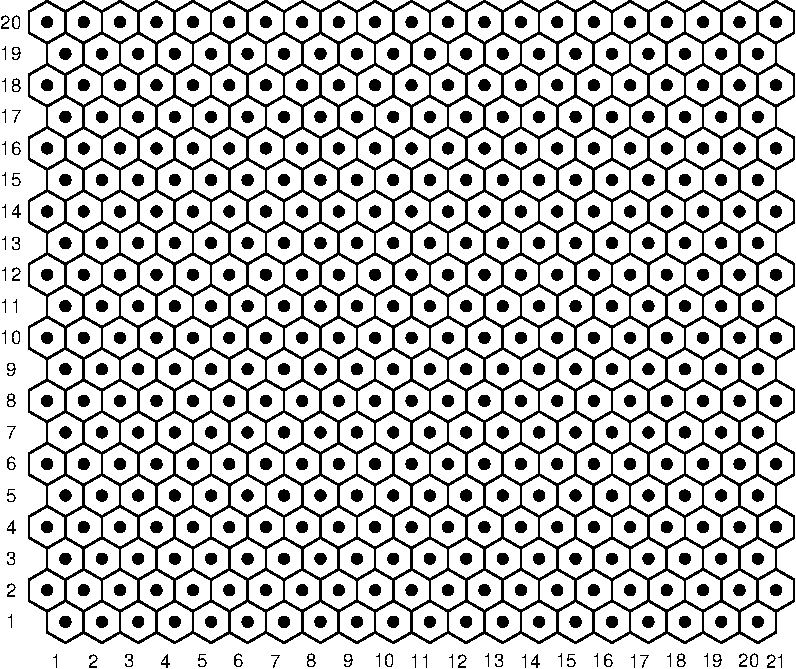
\includegraphics{SOMDisco.README_files/figure-latex/ck-SHGRSOMvislattice-1.pdf}
The SOM visualizations are intended to be setup via a call to \texttt{vis\_som\_setup} then further augmented: in this case with the lattice tiles (whose shape is dependent upon \texttt{lattice\_type}: squares for ``grid'' types, and hexagons for ``hex'' types) and neurons. Most visualization functions have an \texttt{add} argument, which if set to \texttt{FALSE} will call \texttt{vis\_som\_setup} internally (thus bypassing the need to explicitly layer the functions with individual calls).

We set the SOM to monitor every 10,000 steps and train for 500,000 steps:

\begin{Shaded}
\begin{Highlighting}[]
\NormalTok{mysom}\OperatorTok{$}\KeywordTok{set_monitoring_freq}\NormalTok{(}\DecValTok{10000}\NormalTok{)}
\NormalTok{mysom}\OperatorTok{$}\KeywordTok{train_SOM}\NormalTok{(}\DecValTok{500000}\NormalTok{, SHGR}\OperatorTok{$}\NormalTok{X)}
\CommentTok{## SOM Training:}
\CommentTok{## ++ Reporting every 10000, monitoring every 10000steps}
\CommentTok{## 1	2	3	4	5	6	7	8	}
\CommentTok{## 9	10	11	12	13	14	15	16	}
\CommentTok{## 17	18	19	20	21	22	23	24	}
\CommentTok{## 25	26	27	28	29	30	31	32	}
\CommentTok{## 33	34	35	36	37	38	39	40	}
\CommentTok{## 41	42	43	44	45	46	47	48	}
\CommentTok{## 49	50	}
\CommentTok{## End Training (current age = 500000)}
\CommentTok{## ----------------------------------------------------------------}
\CommentTok{## SOM Recall:}
\CommentTok{## ++ finding BMUs of data ... done}
\CommentTok{## ++ building CADJ matrix ... done}
\CommentTok{## ++ setting RF_size ... done}
\CommentTok{## ++ calculating SOM Entropy ... done}
\CommentTok{## ++ populating RF_members ... done}
\CommentTok{## ++ setting lattice fences ... done}
\end{Highlighting}
\end{Shaded}

If monitoring is activated, the quantities discussed in Section WHERE? can be visualized after training:

\begin{Shaded}
\begin{Highlighting}[]
\KeywordTok{vis_som_training}\NormalTok{(}\DataTypeTok{SOM =}\NormalTok{ mysom, }\DataTypeTok{vis.SOM =}\NormalTok{ T, }\DataTypeTok{vis.mtr =}\NormalTok{ T)}
\end{Highlighting}
\end{Shaded}

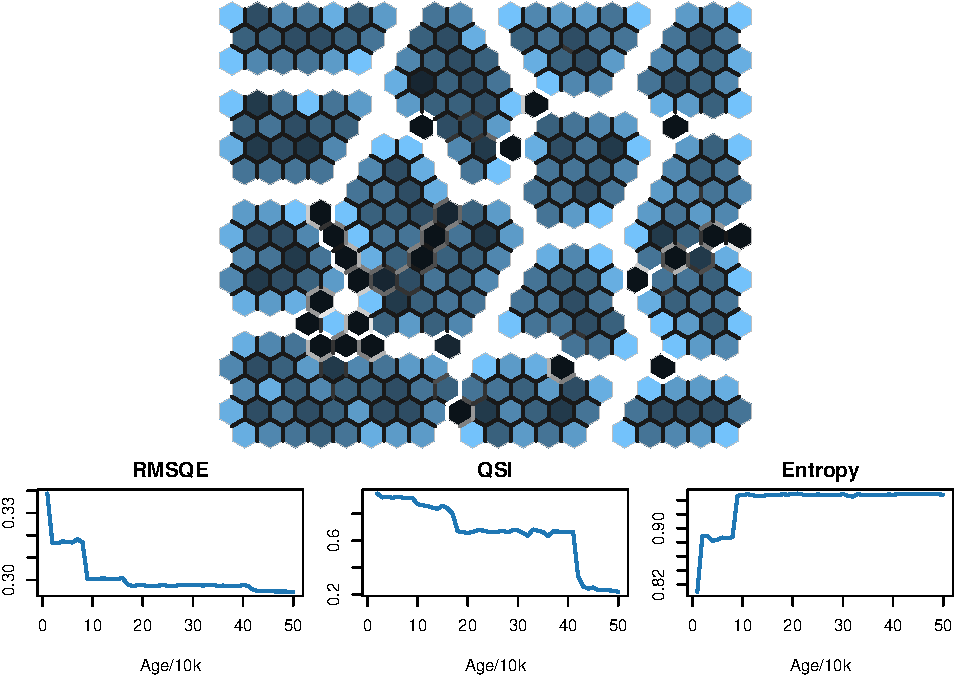
\includegraphics{SOMDisco.README_files/figure-latex/ck-SHGRSOMvismonitor-1.pdf}
The top panel displays a heatmap of the \texttt{RF\_size} of each prototype's Receptive Field. White tiles correspond to empty Receptive Fields, black to low and light blue to high \texttt{RF\_size}; combined, this is the mU-Matrix visualization of {[}\protect\hyperlink{ref-MerenyiJainVillmann}{6}{]} Clusters in these data are readily visible, separated by areas of ``dead'' neurons, which do not represent any training data. The lower panel plots the RMSQE, QSI and Entropy (recorded every 10k training steps) vs training age. While RMSQE and Entropy have been somewhat stable over most of the current age of the SOM QSI has not, indicating further training may be beneficial. We continue training another 500k steps and re-create the monitoring visualization:

\begin{Shaded}
\begin{Highlighting}[]
\CommentTok{# Train another 500k steps and view the resulting age }
\NormalTok{mysom}\OperatorTok{$}\KeywordTok{train_SOM}\NormalTok{(}\DecValTok{500000}\NormalTok{, SHGR}\OperatorTok{$}\NormalTok{X)}
\CommentTok{## SOM Training:}
\CommentTok{## ++ Reporting every 10000, monitoring every 10000steps}
\CommentTok{## 1	2	3	4	5	6	7	8	}
\CommentTok{## 9	10	11	12	13	14	15	16	}
\CommentTok{## 17	18	19	20	21	22	23	24	}
\CommentTok{## 25	26	27	28	29	30	31	32	}
\CommentTok{## 33	34	35	36	37	38	39	40	}
\CommentTok{## 41	42	43	44	45	46	47	48	}
\CommentTok{## 49	50	}
\CommentTok{## End Training (current age = 1000000)}
\CommentTok{## ----------------------------------------------------------------}
\CommentTok{## SOM Recall:}
\CommentTok{## ++ finding BMUs of data ... done}
\CommentTok{## ++ building CADJ matrix ... done}
\CommentTok{## ++ setting RF_size ... done}
\CommentTok{## ++ calculating SOM Entropy ... done}
\CommentTok{## ++ populating RF_members ... done}
\CommentTok{## ++ setting lattice fences ... done}
\NormalTok{mysom}\OperatorTok{$}\NormalTok{age }
\CommentTok{## [1] 1e+06}

\CommentTok{# Visualize Training }
\KeywordTok{vis_som_training}\NormalTok{(}\DataTypeTok{SOM =}\NormalTok{ mysom, }\DataTypeTok{vis.SOM =}\NormalTok{ T, }\DataTypeTok{vis.mtr =}\NormalTok{ T)}
\end{Highlighting}
\end{Shaded}

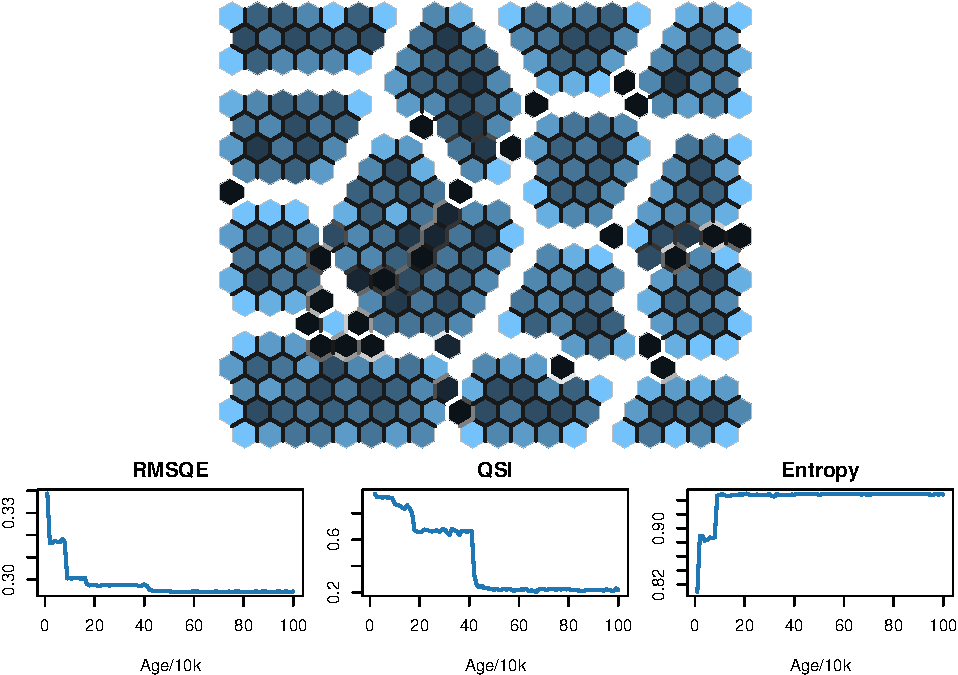
\includegraphics{SOMDisco.README_files/figure-latex/ck-SHGRSOMretrain-1.pdf}
After training we can assess the organization of the lattice by plotting the 100-d SOM prototype vectors in their respective lattice tiles:

\begin{Shaded}
\begin{Highlighting}[]
\CommentTok{# Setup the lattice tiles }
\KeywordTok{vis_som_setup}\NormalTok{(}\DataTypeTok{SOM =}\NormalTok{ mysom, }\DataTypeTok{lattice_coords =}\NormalTok{ T)}
\KeywordTok{vis_som_tiles}\NormalTok{(}\DataTypeTok{SOM =}\NormalTok{ mysom, }\DataTypeTok{add =}\NormalTok{ T)}

\CommentTok{# Add the prototype vectors in lattice situ }
\KeywordTok{vis_som_prototypes}\NormalTok{(}\DataTypeTok{SOM=}\NormalTok{mysom, }\DataTypeTok{add=}\NormalTok{T)}
\end{Highlighting}
\end{Shaded}

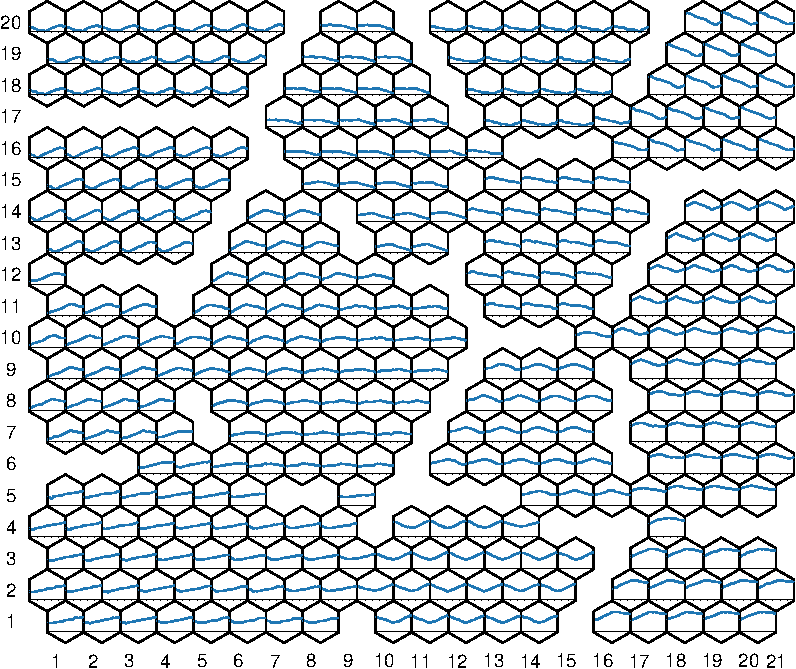
\includegraphics{SOMDisco.README_files/figure-latex/ck-SHGRSOMvisprotos-1.pdf}
Clusters of similar prototype shapes are readily apparent, confirming the organization of this SOM.

We can explore these apparent clusters with the CONNvis visualization which requires the \texttt{TopoRNet} package to be installed as well. Using the \texttt{CONN} matrix just learned we define a \texttt{TRN} object and compute the CONNvis statistics

\begin{Shaded}
\begin{Highlighting}[]
\NormalTok{mytrn =}\StringTok{ }\NormalTok{TRN}\OperatorTok{$}\KeywordTok{new}\NormalTok{()}
\NormalTok{mytrn}\OperatorTok{$}\KeywordTok{set_input_topo}\NormalTok{(mysom}\OperatorTok{$}\NormalTok{W, mysom}\OperatorTok{$}\KeywordTok{CONN}\NormalTok{())}
\CommentTok{## Setting Input Space Topos}
\CommentTok{## ++ storing vertices ... done}
\CommentTok{## ++ storing edge list ... done}
\NormalTok{mytrn}\OperatorTok{$}\KeywordTok{set_output_topo}\NormalTok{(mysom}\OperatorTok{$}\NormalTok{nu_xy, mysom}\OperatorTok{$}\NormalTok{nu_ADJ)}
\CommentTok{## Setting Output Space Topos}
\CommentTok{## ++ storing vertices ... done}
\CommentTok{## ++ storing edge list ... done}
\CommentTok{## ++ computing folding lengths of forward network mapping ... done}
\CommentTok{## ++ computing folding lengths of backward network mapping ...}
\CommentTok{## Warning in mytrn$set_output_topo(mysom$nu_xy, mysom$nu_ADJ): NAs introduced by}
\CommentTok{## coercion to integer range}
\CommentTok{##  done}
\CommentTok{## ++ computing topology preserving radius ... done}
\NormalTok{mytrn}\OperatorTok{$}\KeywordTok{set_CONNvis}\NormalTok{()}
\CommentTok{## CONNvis parameterization:++ computing local ranks ... done}
\CommentTok{## ++ computing local rank stats ... done}
\CommentTok{## ++ computing global ranks ... done}
\CommentTok{## ++ computing global rank stats ... done}
\CommentTok{## ++ computing output topology length stats ... done}
\end{Highlighting}
\end{Shaded}

which are passed, along with our trained SOM, to the function \texttt{vis\_som\_CONNvis}:

\begin{Shaded}
\begin{Highlighting}[]
\KeywordTok{vis_som_CONNvis}\NormalTok{(}\DataTypeTok{SOM =}\NormalTok{ mysom, }\DataTypeTok{TRN =}\NormalTok{ mytrn, }\DataTypeTok{add =}\NormalTok{ F)}
\end{Highlighting}
\end{Shaded}

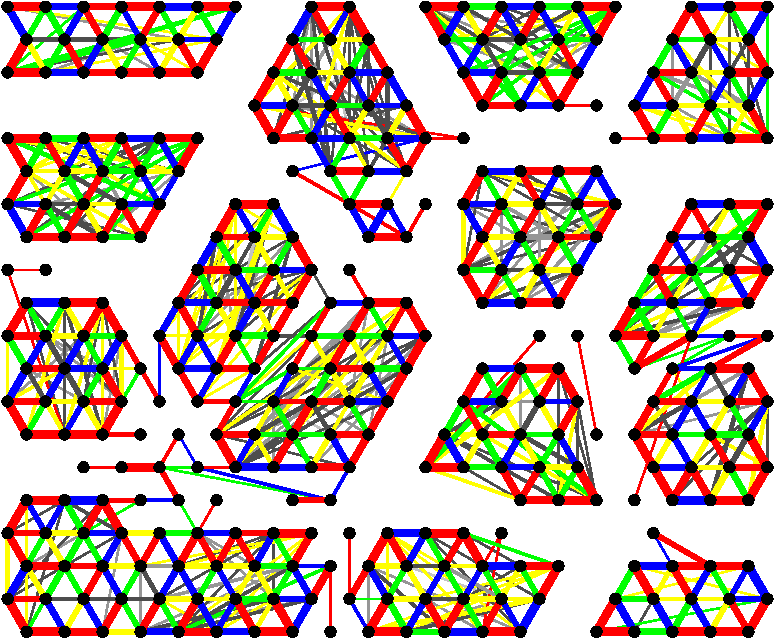
\includegraphics{SOMDisco.README_files/figure-latex/ck-SHGRSOMconnvis-1.pdf}
CONNvis ranks each \texttt{CONN} edge by local and global topological importance, indicated by color (red, blue, green, yellow, grayscale) and line width. As recognized above, many clusters are readily apparent on the SOM with the mU-Matrix visualization alone. CONNvis has further revealed evidence of separation of large clusters in the middle-left and middel-right of the SOM.

Since these training data are labeled we can project the data labels through the learned SOM mapping to expand the CONNvis findings.

\begin{Shaded}
\begin{Highlighting}[]
\NormalTok{mysom}\OperatorTok{$}\KeywordTok{set_RF_label}\NormalTok{(SHGR}\OperatorTok{$}\NormalTok{label)}
\end{Highlighting}
\end{Shaded}

Visualizations involving labels require an additional data frame known as a color table or \texttt{ctab} to function which controls the coloring of each character label found in the dataset. The \texttt{ctab} should be a data frame with columns \texttt{label} (listing the distinct character labels) and \texttt{color} giving a hex color code (or R color name) corresponding to each label. The SHGR data is packaged with the following color table:

\begin{Shaded}
\begin{Highlighting}[]
\KeywordTok{head}\NormalTok{(SHGR}\OperatorTok{$}\NormalTok{ctab)}
\CommentTok{##   label   color}
\CommentTok{## 1     A #0F52BA}
\CommentTok{## 2     B #FF7417}
\CommentTok{## 3     C #4CBB17}
\CommentTok{## 4     D #ED2939}
\CommentTok{## 5     E #B660CD}
\CommentTok{## 6     F #FFF200}
\end{Highlighting}
\end{Shaded}

which can be visualized via

\begin{Shaded}
\begin{Highlighting}[]
\KeywordTok{vis_ctab}\NormalTok{(}\DataTypeTok{ctab=}\NormalTok{SHGR}\OperatorTok{$}\NormalTok{ctab)}
\end{Highlighting}
\end{Shaded}

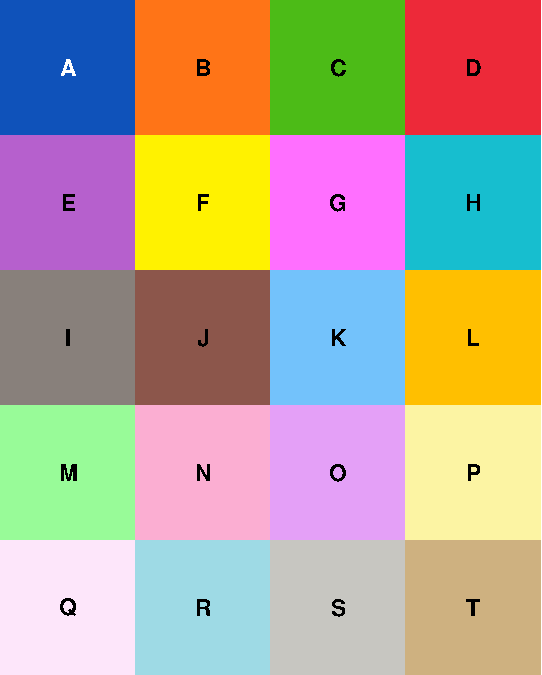
\includegraphics{SOMDisco.README_files/figure-latex/ck-SHGRSOMctab2-1.pdf}

With a color table set, the label distribution in each prototype's Receptive Field can be visualized on the lattice as a proportional pie chart in each lattice tile:

\begin{Shaded}
\begin{Highlighting}[]
\CommentTok{# Setup the lattice tiles}
\KeywordTok{vis_som_setup}\NormalTok{(}\DataTypeTok{SOM =}\NormalTok{ mysom, }\DataTypeTok{lattice_coords =}\NormalTok{ T)}
\KeywordTok{vis_som_tiles}\NormalTok{(}\DataTypeTok{SOM =}\NormalTok{ mysom, }\DataTypeTok{add =}\NormalTok{ T)}

\CommentTok{# View the mapped label distribution}
\KeywordTok{vis_som_labeldist}\NormalTok{(}\DataTypeTok{SOM=}\NormalTok{mysom, }\DataTypeTok{ctab=}\NormalTok{SHGR}\OperatorTok{$}\NormalTok{ctab, }\DataTypeTok{add=}\NormalTok{T)}
\end{Highlighting}
\end{Shaded}

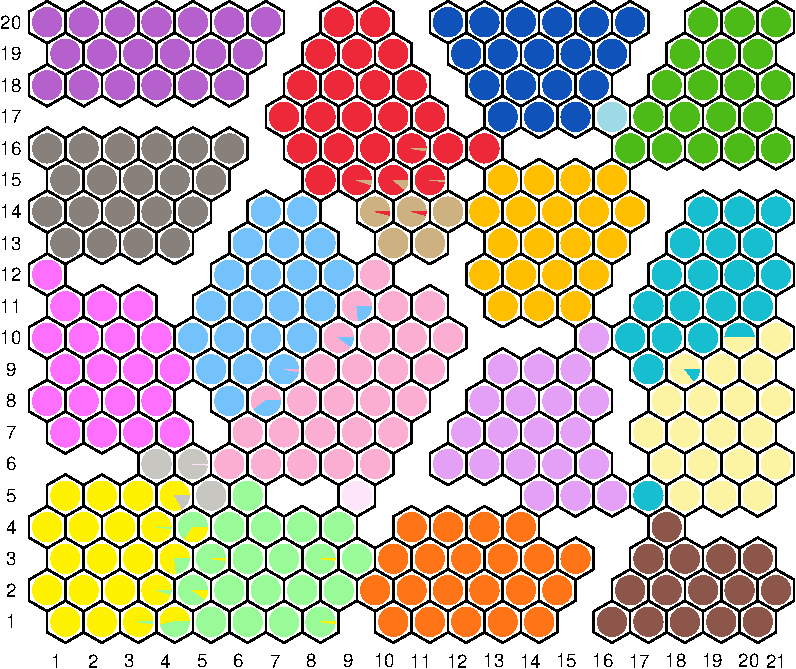
\includegraphics{SOMDisco.README_files/figure-latex/ck-SHGRSOMlabeldist-1.pdf}
The neighborhoods on the SOM appear to be meaningful, with the majority of prototype Receptive Fields containing data of the same label. There is some visible mixing of labels in the RFs of ``boundary prototypes'' which sit between neighboring clusters, which is to be expected for data of any complexity. Often, an analyst may only care about the plurality winning label within each Receptive Field, which can be viewed by ``painting'' the SOM tiles with their corresponding label color, and annotating each tile with its label:

\begin{Shaded}
\begin{Highlighting}[]
\CommentTok{# Setup the lattice tiles, colored by prototype label }
\KeywordTok{vis_som_setup}\NormalTok{(}\DataTypeTok{SOM =}\NormalTok{ mysom, }\DataTypeTok{lattice_coords =}\NormalTok{ T)}
\KeywordTok{vis_som_label}\NormalTok{(}\DataTypeTok{SOM =}\NormalTok{ mysom, }\DataTypeTok{ctab =}\NormalTok{ SHGR}\OperatorTok{$}\NormalTok{ctab, }\DataTypeTok{add =}\NormalTok{ T)}

\CommentTok{# Annotate the tiles with the label }
\KeywordTok{vis_som_annotate}\NormalTok{(}\DataTypeTok{SOM =}\NormalTok{ mysom, }\DataTypeTok{add =}\NormalTok{ T, }\DataTypeTok{text =}\NormalTok{ mysom}\OperatorTok{$}\NormalTok{RF_label)}
\end{Highlighting}
\end{Shaded}

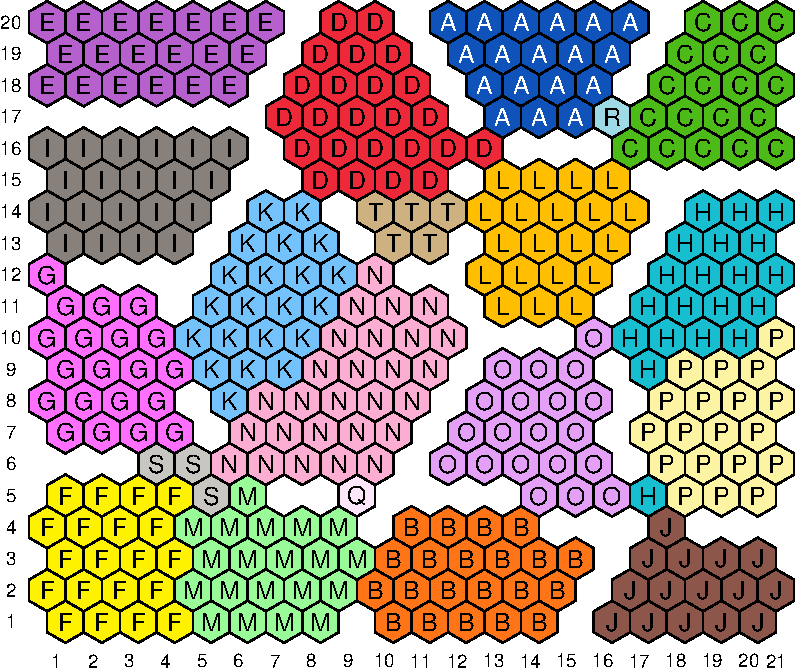
\includegraphics{SOMDisco.README_files/figure-latex/ck-SHGRSOMlabel-1.pdf}
The propagated labels display roughly the same prototype clustering as suggested by the CONNvis above, confirming both our suggested clustering and the quality of the SHGR labeling.

\hypertarget{references}{%
\section*{References}\label{references}}
\addcontentsline{toc}{section}{References}

\hypertarget{refs}{}
\leavevmode\hypertarget{ref-Kohonen2001}{}%
{[}1{]} T. Kohonen, \emph{Self-organizing maps}. Springer, 2000.

\leavevmode\hypertarget{ref-DeSieno1988}{}%
{[}2{]} D. DeSieno, ``Adding a conscience to competitive learning,'' in \emph{IEEE international conference on neural networks}, 1988, vol. 1, pp. 117--124.

\leavevmode\hypertarget{ref-TasdemirMerenyi2009}{}%
{[}3{]} K. Taşdemir and E. Merényi, ``Exploiting data topology in visualization and clustering of self-organizing maps,'' \emph{IEEE Transactions on Neural Networks}, vol. 20, no. 4, pp. 549--562, 2009.

\leavevmode\hypertarget{ref-MartinetzSchulten1994}{}%
{[}4{]} T. Martinetz and K. Schulten, ``Topology representing networks,'' \emph{Neural Networks}, vol. 7, no. 3, pp. 507--522, 1994.

\leavevmode\hypertarget{ref-UMatrix}{}%
{[}5{]} A. Ultsch and H. P. Siemon, ``Kohonen's self organizing feature maps for exploratory data analysis,'' in \emph{Proceedings of the international neural network conference (innc-90), paris, france, july 9--13, 1990 1. Dordrecht, netherlands}, 1990, vol. 1, pp. 305--308.

\leavevmode\hypertarget{ref-MerenyiJainVillmann}{}%
{[}6{]} E. Merényi, A. Jain, and T. Villmann, ``Explicit magnification control of self-organizing maps for `forbidden' data,'' \emph{IEEE Transactions on Neural Networks}, vol. 18, no. 3, pp. 786--797, 2007.

\end{document}
